% allgem. Dokumentenformat
\documentclass[a4paper,12pt,headsepline]{scrartcl}
%Variablen welche innerhalb der gesamten Arbeit zur Verfügung stehen sollen
\newcommand{\titleDocument}{Automatische Erkennung von Arnika in Drohnenluftbildern}
\newcommand{\subjectDocument}{Bachelorarbeit im Studiengang Umweltnaturwissenschaften}



%Entwickung einer Anwendungssoftware zum Monitoring von Arnika Blumen durch die Auswertung von Luftbildern von Drohnen


% weitere Pakete
% Grafiken aus PNG Dateien einbinden
\usepackage{graphicx}
\usepackage{subfigure}
\usepackage{wrapfig}

% Deutsche Sonderzeichen benutzen 
\usepackage{ngerman}

% deutsche Silbentrennung
\usepackage[ngerman]{babel}

\usepackage{blindtext}
% Eurozeichen einbinden
%\usepackage[right]{eurosym}

% Umlaute unter UTF8 nutzen
\usepackage[utf8]{inputenc}

% Zeichenencoding
\usepackage[T1]{fontenc}

% \usepackage{lmodern}
\usepackage{fix-cm}

% floatende Bilder ermöglichen
%\usepackage{floatflt}
\usepackage{float}

% mehrseitige Tabellen ermöglichen
\usepackage{longtable}
%\usepackage{tabularx}

% Unterstützung für Schriftarten
%\newcommand{\changefont}[3]{ 
%\fontfamily{#1} \fontseries{#2} \fontshape{#3} \selectfont}
\usepackage{mathptmx} % Hier steckt Times drin
\usepackage[scaled=0.86]{helvet}
\usepackage{courier}

% Packet für Seitenrandabständex und Einstellung für Seitenränder
\usepackage{geometry}
\geometry{left=3.5cm, right=2cm, top=2.5cm, bottom=2cm}

% Paket für Boxen im Text
\usepackage{fancybox}

% bricht lange URLs "schoen" um
\usepackage[hyphens,obeyspaces,spaces]{url}

% Paket für Textfarben
\usepackage{color}

% Mathematische Symbole importieren
\usepackage{amssymb}

% auf jeder Seite eine Überschrift (alt, zentriert)
%\pagestyle{headings}

% erzeugt Inhaltsverzeichnis mit Querverweisen zu den Kapiteln (PDF Version)
\usepackage[pdfborderstyle={/S/U/W 1},bookmarksnumbered,pdftitle={\titleDocument},hyperfootnotes=false]{hyperref} 
%\hypersetup{colorlinks, citecolor=green, linkcolor=black, urlcolor=red}
%\hypersetup{colorlinks, citecolor=black, linkcolor=black, urlcolor=black}

% neue Kopfzeilen mit fancypaket
\usepackage{fancyhdr} %Paket laden
\pagestyle{fancy} %eigener Seitenstil
\fancyhf{} %alle Kopf- und Fußzeilenfelder bereinigen
\fancyhead[L]{\nouppercase{\leftmark}} %Kopfzeile links
\fancyhead[C]{} %zentrierte Kopfzeile
\fancyhead[R]{\thepage} %Kopfzeile rechts
\renewcommand{\headrulewidth}{0.4pt} %obere Trennlinie
%\fancyfoot[C]{\thepage} %Seitennummer
%\renewcommand{\footrulewidth}{0.4pt} %untere Trennlinie

% für Tabellen
\usepackage{array}

% Runde Klammern für Zitate
\usepackage[authoryear,round]{natbib}

% Festlegung Art der Zitierung - Havardmethode: Abkuerzung Autor + Jahr
\bibliographystyle{plainnat}
\setcitestyle{notesep={: }, yysep={,}}
% Schaltet den zusätzlichen Zwischenraum ab, den LaTeX normalerweise nach einem Satzzeichen einfügt.
\frenchspacing

% Paket für Zeilenabstand
\usepackage{setspace}

% für Bildbezeichner
\usepackage{capt-of}
\usepackage{caption}
\captionsetup[figure]{labelfont={sf,sc}, textfont=sf}
\captionsetup[table]{labelfont={sf,sc}, textfont=sf}

% für Stichwortverzeichnis
\usepackage{makeidx}

% für Listings
\usepackage{listings}
\lstset{numbers=left, numberstyle=\tiny, numbersep=5pt, keywordstyle=\color{black}\bfseries, stringstyle=\ttfamily,showstringspaces=false,basicstyle=\footnotesize,captionpos=b}
\lstset{language=python}

\usepackage[edges]{forest}
\definecolor{folderbg}{RGB}{124,166,198}
\definecolor{folderborder}{RGB}{110,144,169}
\newlength\Size
\setlength\Size{4pt}
\tikzset{%
  folder/.pic={%
    \filldraw [draw=folderborder, top color=folderbg!50, bottom color=folderbg] (-1.05*\Size,0.2\Size+5pt) rectangle ++(.75*\Size,-0.2\Size-5pt);
    \filldraw [draw=folderborder, top color=folderbg!50, bottom color=folderbg] (-1.15*\Size,-\Size) rectangle (1.15*\Size,\Size);
  },
  file/.pic={%
    \filldraw [draw=folderborder, top color=folderbg!5, bottom color=folderbg!10] (-\Size,.4*\Size+5pt) coordinate (a) |- (\Size,-1.2*\Size) coordinate (b) -- ++(0,1.6*\Size) coordinate (c) -- ++(-5pt,5pt) coordinate (d) -- cycle (d) |- (c) ;
  },
}
\forestset{%
  declare autowrapped toks={pic me}{},
  pic dir tree/.style={%
    for tree={%
      folder,
      font=\ttfamily,
      grow'=0,
    },
    before typesetting nodes={%
      for tree={%
        edge label+/.option={pic me},
      },
    },
  },
  pic me set/.code n args=2{%
    \forestset{%
      #1/.style={%
        inner xsep=2\Size,
        pic me={pic {#2}},
      }
    }
  },
  pic me set={directory}{folder},
  pic me set={file}{file},
}

\usepackage{todonotes}
\newcommand{\tg}[1]{\todo[color=green!40]{#1}}
\newcommand{\fio}[1]{\todo[color=blue!40]{#1}}

% Indexerstellung
\makeindex

% Abkürzungsverzeichnis
\usepackage[german]{nomencl}
\let\abbrev\nomenclature

% Abkürzungsverzeichnis LiveTex Version
\renewcommand{\nomname}{Abkürzungsverzeichnis}
\setlength{\nomlabelwidth}{.25\hsize}
\renewcommand{\nomlabel}[1]{#1 \dotfill}
\setlength{\nomitemsep}{-\parsep}
\makenomenclature
%\makeglossary

% Abkürzungsverzeichnis TeTEX Version
% \usepackage[german]{nomencl}
% \makenomenclature
% %\makeglossary
% \renewcommand{\nomname}{Abkürzungsverzeichnis}
% \setlength{\nomlabelwidth}{.25\hsize}
% \renewcommand{\nomlabel}[1]{#1 \dotfill}
% \setlength{\nomitemsep}{-\parsep}

% Disable single lines at the start of a paragraph (Schusterjungen)
\clubpenalty = 10000
% Disable single lines at the end of a paragraph (Hurenkinder)
\widowpenalty = 10000
\displaywidowpenalty = 10000

\begin{document}
% hier werden die Trennvorschläge inkludiert
%hier müssen alle Wörter rein, welche Latex von sich auch nicht korrekt trennt bzw. bei denen man die genaue Trennung vorgeben möchte
\hyphenation{
Film-pro-du-zen-ten
Lux-em-burg
Soft-ware-bau-steins
zeit-in-ten-siv
durch-blu-tungs-stei-gernd
Wild-pflück-un-gen
Bun-des-art-en-schutz-ver-ord-nung
Bun-des-na-tur-schutz-ge-setz
}



%Schriftart Helvetica
%\changefont{phv}{m}{n}

% Leere Seite am Anfang
\newpage
\thispagestyle{empty} % erzeugt Seite ohne Kopf- / Fusszeile
\section*{ }

% Titelseite %
% das Papierformat zuerst
%\documentclass[a4paper, 11pt]{article}

% deutsche Silbentrennung
%\usepackage[ngerman]{babel}

% wegen deutschen Umlauten
%\usepackage[ansinew]{inputenc}

% hier beginnt das Dokument
%\begin{document}


\thispagestyle{empty}

%\begin{figure}[t]
% \includegraphics[width=0.6\textwidth]{abb/fh_koeln_logo}
%\end{figure}

\begin{figure}[t]
 \begin{flushright}
 
\includegraphics{abb/unilogo}
 \end{flushright}
\end{figure}

\begin{verbatim}

\end{verbatim}

\begin{center}
\Large{Fakultät für Umwelt und natürliche Ressourcen}
\end{center}
\begin{verbatim}

\end{verbatim}
\begin{center}
\doublespacing
\textbf{\LARGE{\titleDocument}}\\
\singlespacing
\begin{verbatim}

\end{verbatim}
\textbf{{~\subjectDocument~}}
\end{center}
\begin{verbatim}

\end{verbatim}
\begin{center}

\end{center}
\begin{verbatim}

\end{verbatim}
\begin{center}
\textbf{zur Erlangung des akademischen Grades \\ Bachelor of Science}
\end{center}
\begin{verbatim}



\end{verbatim}
\begin{flushleft}
\begin{tabular}{llll}
& & \\
\textbf{Autorin:} & & Anna Tenberg & \\
& & MatNr. 3327360 & \\
& & \\
\textbf{Version vom:} & & \today &\\
& & \\
\textbf{1. Betreuer:} & & Dr.-Ing. Holger Weinacker &\\
\textbf{2. Betreuer:} & & Prof. Dr. Albert Reif &\\
\end{tabular}
\end{flushleft}


% römische Numerierung
%\pagenumbering{arabic}

% 1.5 facher Zeilenabstand
\onehalfspacing

% Sperrvermerk
%\section*{Sperrvermerk}
\textcolor{red}{
Die vorliegende Arbeit beinhaltet interne und vertrauliche Informationen der Firma <Firmenname>.
Die Weitergabe des Inhalts der Arbeit im Gesamten oder in Teilen sowie das Anfertigen
von Kopien oder Abschriften - auch in digitaler Form - sind grundsätzlich untersagt.
Ausnahmen bedürfen der schriftlichen Genehmigung der Firma <Firmenname>.
}

% Einleitung / Abstract
\section*{Zusammenfassung}


%\begin{verbatim}

%

%\end{verbatim}

\section*{Abstract}


% einfacher Zeilenabstand
\singlespacing

% Inhaltsverzeichnis anzeigen
\newpage
\tableofcontents

% das Abbildungsverzeichnis
\newpage
% Abbildungsverzeichnis soll im Inhaltsverzeichnis auftauchen
\addcontentsline{toc}{section}{Abbildungsverzeichnis}
% Abbildungsverzeichnis endgueltig anzeigen
\listoffigures

% das Tabellenverzeichnis
%\newpage
% Abbildungsverzeichnis soll im Inhaltsverzeichnis auftauchen
\addcontentsline{toc}{section}{Tabellenverzeichnis}
% \fancyhead[L]{Abbildungsverzeichnis / Abkürzungsverzeichnis} %Kopfzeile links
% Abbildungsverzeichnis endgueltig anzeigen
\listoftables

\addcontentsline{toc}{section}{Todoliste}
\listoftodos
%% WORKAROUND für Listings
%\makeatletter% --> De-TeX-FAQ
%\renewcommand*{\lstlistoflistings}{%
%  \begingroup
%    \if@twocolumn
%      \@restonecoltrue\onecolumn
%    \else
%      \@restonecolfalse
%    \fi
%    \lol@heading
%    \setlength{\parskip}{\z@}%
%    \setlength{\parindent}{\z@}%
%    \setlength{\parfillskip}{\z@ \@plus 1fil}%
%    \@starttoc{lol}%
%    \if@restonecol\twocolumn\fi
%  \endgroup
%}
%\makeatother% --> \makeatletter
% das Listingverzeichnis
%\newpage
% Listingverzeichnis soll im Inhaltsverzeichnis auftauchen
% \addcontentsline{toc}{section}{Listingverzeichnis}
% %\fancyhead[L]{Abbildungs- / Tabellen- / Listingverzeichnis} %Kopfzeile links
% \renewcommand{\lstlistlistingname}{Listingverzeichnis}
% \lstlistoflistings
%%%%

% das Abkürzungsverzeichnis
\newpage
% Abkürzungsverzeichnis soll im Inhaltsverzeichnis auftauchen
\addcontentsline{toc}{section}{Abkürzungsverzeichnis}
% das Abkürzungsverzeichnis entgültige Ausgeben
%\fancyhead[L]{Abkürzungsverzeichnis} %Kopfzeile links
\nomenclature{BfN}{Bundesamt für Naturschutz}
\nomenclature{BRD}{Bundesrepublik Deutschland}
\nomenclature{DDR}{Deutsche Demokratische Republik}
\nomenclature{RL}{Rote Liste gefährdeter Tiere, Pflanzen und Pilze Deutschlands}
\nomenclature{SL}{Sesquinterpenlactone}
\nomenclature{FNR}{Fachagentur Nachwachsender Rohstoffe e.V.}
\nomenclature{FFH-Richtlinie}{Fauna-Flora-Habitat-Richtlinie}
\nomenclature{PSF}{Python Software Foundation}
\nomenclature{ALU-FR}{Albert-Ludwigs-Universität Freiburg}
\nomenclature{BFA}{Bioflora Apuseni}
\nomenclature{USAMV}{Universität für Agrarwissenschaften und Tiermedizin Cluj-Napoca}
\nomenclature{BMBF}{Bundesministerium für Bildung und Forschung}
\nomenclature{WWF}{World Wide Fund For Nature}
\nomenclature{UAV}{Unmanned Aircraft Vehicels}
\nomenclature{UAS}{Unmanned Aircraft Systems}
\nomenclature{DOM}{Digitales Oberflächenmodell}
\nomenclature{DGM}{Digitales Geländemodell}
\nomenclature{GNSS}{Globales Navigationssatellitensystem}
\nomenclature{RTK}{real-time kinematics}
\nomenclature{PPK}{post-processing kinematics}
\nomenclature{GUI}{graphische Benutzeroberfläche}

\printnomenclature

% Definiert Stegbreite bei zweispaltigem Layout
\setlength{\columnsep}{25pt}

%%%%%%% EINLEITUNG %%%%%%%%%%%%
%\twocolumn
\newpage
%\fancyhead[L]{\nouppercase{\leftmark}} %Kopfzeile links

% 1,5 facher Zeilenabstand
\onehalfspacing

% einzelne Kapitel
\section{Einleitung}\label{einleitung}

\begin{enumerate}
  \item Einleitung
  \begin{itemize}
    \item Problemstellung und Zielsetzung
  \end{itemize}
  
  \item Hintergrund
  \\
    - Arnika
    \begin{itemize}
      \item medizinische Nutzung
      \item ökologische Besonderheiten
      \item nachhaltige Ernte
    \end{itemize}
    - Projekt Apuseni
    \begin{itemize}
      \item Projektpartner
      \item Ökologischer Hintergrund
      \item Vorgehensweise
      \item Drohneneinsatz zur Fernerkundung
    \end{itemize}
    - Testflüge im Schwarzwald (Methoden?)
    \begin{itemize}
        \item Welche Art von Drohne (Schnelligkeit/Höhe vs Bildqualität)
        \item Warum Monitoring mit Hilfe von Drohnen (Vorteile etc)
        \item Durchführung (Flugplanung und Beispielbilder beschreiben)
        \item entstandene Bilder beurteilen, Erfolgreich?
        
    \end{itemize}
    
  \item Monitoringsoftware
    
      - Programmiersprache %(Verweis auf Einstiegsmöglichkeit in die verwendete Programmiersprache-> Anhang)
      
      - Anwendungsbereich

      - Methoden %Vorgehensweise
        \begin{itemize}
        \item Parameterbeschreibung
        \end{itemize}
      - Programmaufbau %(Flow-chart und Beschreibung der einzelnen Bestandteile und der Verknüpfungen zwischen den Modulen)

      - Implementierung / Aufruf
        \begin{itemize}
          \item Hard- und Softwarevoraussetzungen
          \item In- und Output-Dateien %und deren Formate      
        \end{itemize}
      %\item Einbindungsmöglichkeiten in andere Anwendungen
      %\item Bei komplexen Berechnungsverfahren Beschreibung der Algorithmen und Literaturhinweise zu den Quellen der Verfahren

    
    
  \item Ergebnisse
    \begin{itemize}
      \item Auswertung
      \item Alle Ergebnisse werden hinsichtlich der Zielsetzung (Anfangshypothesen)
bewertet
      \item Alle Ergebnisse werden mit relevanter Literatur verglichen und bewertet
      \item Verbesserungsmöglichkeiten
      \item Schwierigkeiten Probleme (-> Verwechslungspotential Arnika?) 
      \item Die eigenen Ergebnisse werden nicht über- oder unterbewertet
    \end{itemize}
  \item Diskussion?
  \item Schluss
    \begin{itemize}
      \item Zusammenfassung
      \item Fazit Schlussfolgerungen
      \item Rückbezug auf Ziele
      \item Evaluation
      \item Ausblick
    \end{itemize}
  

\end{enumerate}

\subsection{Ziele}\label{ziele}

Das Ziel der Arbeit ist die Entwicklung einer Anwendungssoftware, die das Monitoring von Arnika Pflanzen erleichtert. Das Programm wird zur Analyse von Luftaufnahmen, die durch Drohnen gemacht wurden, verwendet. Dabei sollen visuelle Erkenntnisse über die Quantität von Arnika Blüten in den Fotos gewonnen werden.
Die Software soll auf Daten mit unterschiedlicher Qualität und Größe anwendet werden können. 


%ich muss konkretisieren dass meine "Anwendungssoftware" nicht gleich die Software des Projektes ist. also kurz meine Relation zu dem Projekt sagen und eine kritische EInschätzung was mein Programm kann oder was nicht.
%Und zwar schon in der Einleitung. Und dann dass ich dem projekt zuarbeite, bzw. 

\newpage
\section{Hintergrund}\label{kapitel1}

Beschreibung warum die subsections Teil der Arbeit sind. 

%- Beschreibung Arnika (Zusammenfassung)
%- Botanische Beschreibung 
%- Medizinische Nutzung
%   - Umstrittene Nutzung innerer Anwendung bei Herz- Kreislaufbeschwerden (Goethe Zitat)
% - Naturschutzstatus
% - Anbau und Schwierigkeiten -> weitere Notwendigkeit der nachhaltigen Wildsammlungen v.A. in Rumänien
\subsection{\textit{Arnica montana}}

\begin{quotation}
„Wenn man nur eine einzige Pflanze in der Hausapotheke haben könnte, so würde ich zu Arnika raten.“ \citep[S. 186]{Sommer2011}
\end{quotation}

\textit{Arnica montana}, auch „Bergwohlverleih“ genannt, ist eine Arzneipflanze, die seit Jahrhunderten wegen ihrer tiefen Heilwirkung bekannt ist und verwendet wird. Die vermutlich erste Erwähnung fand Arnika bei Hildegard \citet{Bingen2007}, die sie in ihrem Buch von den Pflanzen von 1151–1158 „Woluis gelegena“ nennt. Sie beschreibt Arnika als Liebesmittel zur äußeren Anwendung. Arnika sei „sehr warm und hat eine giftige Wärme in sich“. Die erste Erwähnung als Arzneipflanze findet sich 1588 im Kräuterhandbuch von Tabernaemontanus, eigentlich Jacob Theodor aus Bergzabern. In der breiten Bevölkerung wird Arnika ab dem 18. Jahrhundert bei Krankheiten und Beschwerden eingesetzt. Deshalb tauchte sie auch im Herbarium Backwellium von Elizabeth \citet{Blackwell1757} und dem Medizinal von Franz Eugen \citet{Kohler1887} auf (Siehe Abbildung~\ref{fig:Zeichnung}, S.\pageref{fig:Zeichnung}).

\begin{figure}[htb]
    \subfigure[]{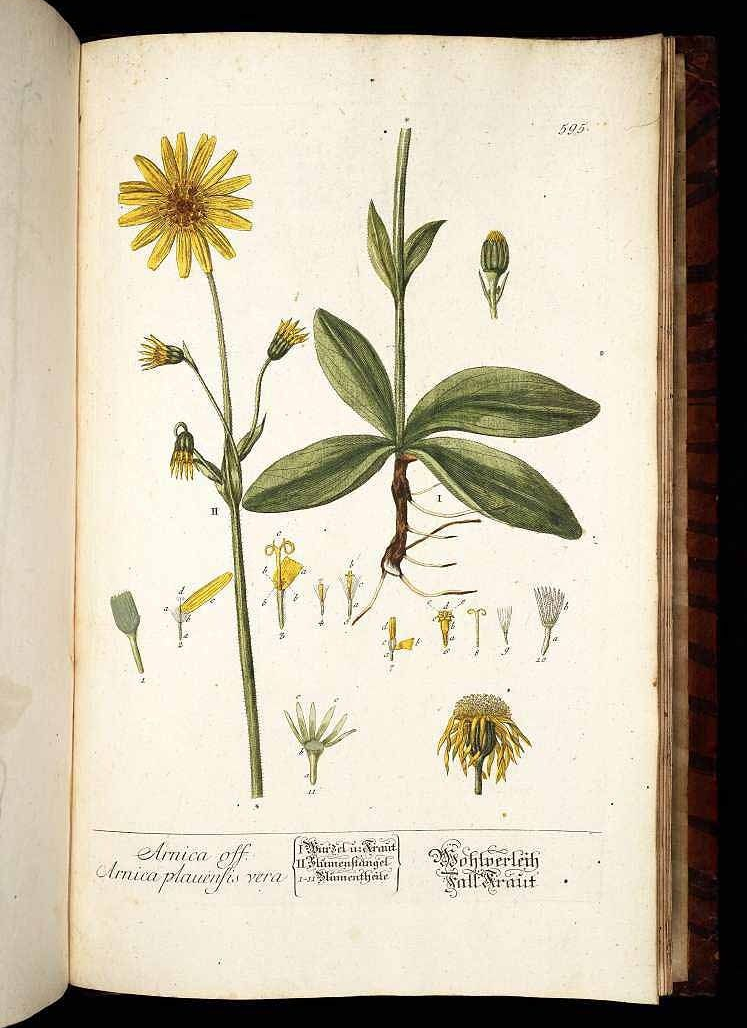
\includegraphics[width=0.49\textwidth]{abb/herbarium-blackwell}}
    \subfigure[]{\includegraphics[width=0.49\textwidth]{abb/Koehler-medizinal-pflanzen}}
\caption{\textit{Arnica montana} aus \citet{Blackwell1757} (a) und \citet{Kohler1887} (b)}
  \label{fig:Zeichnung}
\end{figure}

Aufgrund ihrer fiebersenkenden Wirkung galt sie lange als das „Chinin der armen Leute“. Sebastian Kneipp hat angeblich täglich mit Arnikatee gegurgelt. „Arnika ist nicht mit Gold zu bezahlen“, soll er gesagt haben. Auch Johann Wolfgang nutzte Arnika: Er erholte sich 1823, 10 Jahre vor seinem Tod, vermutlich von einem Herzinfakt durch eine Tasse Arnikatee \citep[vgl.][S.56]{Franke2012}.

Die \textit{Arnica montana} zählt zu den Korbblütern (botanisch Asteraceae oder Compositae) und ist eine mehrjährige Staudenpflanze, die meist eine maximale Höhe von 30 bis 60 cm erreicht. Die behaarten Blätter haben eine elliptische Form und sind in am Boden anliegenden Rosetten angeordnet. Zusätzlich hat die \textit{Arnica montana} ein bis drei gegenständige Stängelblätter \citep[vgl.][]{Wyk2015, FNR2013}. Eine Pflanze besitz ein bis drei 5-8 cm breite Blütenköpfe mit gelb-orangen dreigezähnten Zungen- oder Röhrenblüten. Die Blütezeit ist von Juni bis August. \textit{Arnica montana} steht auf Magerrasen, Wiesen, trockenen Mooren und Heiden, sowie in lichten Nadelwäldern. Sie ist als Wildpflanze bis in die alpine Stufe weiter Teile Europas zu finden \citep[vgl.][]{Schoenfelder2011, FNR2013}.

Es gibt zwei Unterarten (subsp.) bei der \textit{Arnica montana}: \textit{montana} und \textit{atlantica}. Die \textit{Arnica montana ssp. montana} ist die sogenannte alpine Arnika, die vor allem in Höhenlagen Mittel und Osteuropas zu finden ist. Die \textit{Arnica montana ssp. atlantica}, wird auch spanische Arnika genannt und ist nur in den französischen und spanischen Pyrenäen und im Norden Spaniens und Portugals zu finden. Die Blüten der spanischen Arnika sind etwas kleiner und heller als bei der alpinen Arnika, sie ähnelt damit der nordamerikanischen \textit{Arnica chamissonis} (Siehe Abbildung~\ref{fig:Unterarten}, S.\pageref{fig:Unterarten}) \citep[vgl.][S. 61]{Franke2012}.

\begin{figure}[htb]
 \centering
 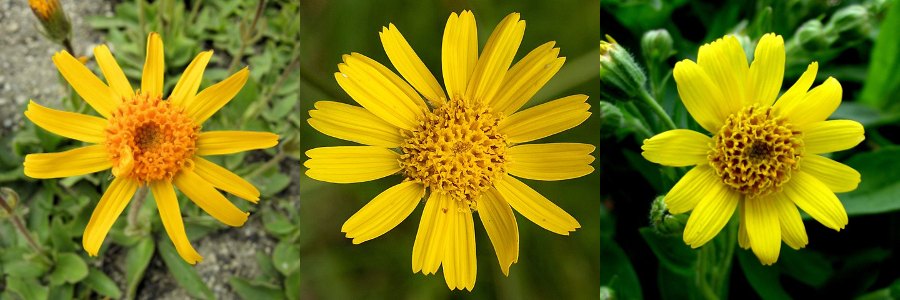
\includegraphics[width=\textwidth,angle=0]{abb/Arnika/arnica-900x300}
 \caption{v.l.n.r.: alpine Arnika \citep{Moro2019}, spanische Arnika \citep{Pereira2019} und nordamerikanische Wiesen-Arnika \citep{Rowlin2019}}
\label{fig:Unterarten}
\end{figure}

\subsubsection{Medizinische Wirkung}

Die ganze Arnika-Pflanze enthält Wirkstoff. Früher wurden vor allem Wurzeln zur medizinischen Anwendung genutzt, heute meist nur die Blüten, auch Arnicae Flos oder Flores Arnica (montanae) genannt \citep[vgl.][S. 144 f.]{Roth2012}. Die Hauptwirkstoffe der Blüten (0,1-0,5\%) sind die Sesquinterpenlactone (SL) Helenalin und Dihydrohelenalin sowie deren Ester. SL können kovalente Bindungen mit Proteinen eingehen und so deren Aktivität verändert \citep[vgl.][S. 62]{Wyk2015}. Durch Helenalin kann die Vermehrung von Mikroorganismen gehemmt werden, was Entzündungen entgegen wirkt \citep[vgl.][S. 32 f.]{FNR2013}. \citet[S. 73 f.]{Schoenfelder2011} schreibt: „Die Helenalinester sind gleichzeitig für die Nebenwirkungen verantwortlich, vor allem die relativ häufig auftretenden allergisch bedingten Hautreaktionen nach äußerer Anwendung“. Andere Inhaltsstoffe von Arnika sind Flavone (gelbe Pflanzenfarbstoffe) und Flavonoide. Auf Flavonoide lässt sich ebenfalls die entzündungshemmende Eigenschaft von Arnika zurück verfolgen. Außerdem enthält \textit{Arnica montana} verschiedene ätherische Öle, Trierpenalkohole, Phenolcarbonsäuren und Polysaccharide \citep[vgl.][]{Wyk2015, Schoenfelder2011}. Insgesamt gibt es bei dem Inhaltsstoffen und deren Mengen erhebliche Schwankungen je nach Standort \citep[vgl.][S. 144 f.]{Roth2012}.

% -Wirkung und äußere Anwendung
Arnika wirkt entzündungshemmend, schmerzstillend, antiseptische, durchblutungssteigernd und wundheilend. Traditionell wird Arnika als alkoholische Tinktur, auch „Arnika-Schnaps” genannt, verdünnt zum Einreiben oder für Umschläge verwendet. Im Handel gibt es heute daneben vor allem Salben und Cremes sowie homöopathische Zubereitungen \citep[vgl.][S. 32 f.; S. 399]{FNR2013, Prentner2017}. Angewendet wird Arnika äußerlich zur Behandlung von stumpfen Verletzungen, Hämatomen, Quetschungen, Ödemen, Verrenkungen, Verstauchungen, Muskelschmerzen, Gelenkschmerzen, Venenbeschwerden oder rheumatischen Beschwerden. Auch bei Schleimhautentzündungen in Mund und Rachen, so wie Insektensticken oder Sonnenbrand kann Arnika angewendet werden \citep[vgl.][]{Roth2012, Prentner2017, Wyk2015, FNR2013, Schoenfelder2011}.

%Studie zur Homöopatischen Wirksamkeit im vergleich zu diclofenac (orale Einnahme) ???

%Nebenwirkungen und Allergiepotential
Bei längerer Anwendung an geschädigter Haut oder bei zu hoher Konzentration kann es Nebenwirkungen in Form von Ekzemen, ödematöser Dermatitis oder eiterhaltiger Bläschenbildung, bis hinzu Nekrotisierung, kommen \citep[vgl.][S. 144 f.]{Roth2012}. Eine Einnahme kann beim Mensch zur Reizung des Magen-Darm-Traktes, Kopfschmerz, Erschwerung der Atmung, starkem Herzklopfen und Schwindelgefühl führen \citep[vgl.][S. 144 f., S.178]{Roth2012, Schoenfelder2015}. Beim Tier beschreiben \citet{Roth2012} ähnliche Symptome: „Wirkungen auf Nerven- und Gefäßsystem, Beschleunigung der Atmung, Vermehrung der Schweiß- und Harnabsonderung“. Zusätzlich zu den Nebenwirkungen kann Arnika kontaktallergische Reaktionen auslösen, diese sind auf das Helenalin zurückzuführen. Bei einer bekannten Überempfindlichkeit gegen Korbblüter sollte Arnika nicht angewendet werden \citep[vgl.]{Schoenfelder2015, FNR2013, Wyk2015}. 
Die spanische Arnika hat ein wesentlich geringeres Allergiepotenzial, da sie statt Helenalin Dihydrohelenalin enthält. Einigen Studien zufolge ist das Allergie und Nebenwirkungsrisiko insgesamt bei Arnika gering, wenn eine korrekte Anwendung und niedrige Dosierung erfolgt. Eine Untersuchung der Allergie-Forschungsgruppe der Hautklinik Freiburg hat sogar ergeben, dass bei der äußeren Anwendung von Arnika nicht nur keine kontaktallergene Reaktionen festgestellt werden konnten, sondern die entzündungshemmende Wirkung der Arnika einer Allergie und möglichen Schwellungen entgegenwirkt \citep[vgl.][S. 448]{Buehring2014}

% innere Anwendung
Die innere Anwendung oder Einnahme von Arnika ist sehr umstritten und wird heute meist abgelehnt. \citet[S. 144 f.]{Roth2012} und \citet[S. 62]{Wyk2015} warnen aufgrund von toxischen Nebenwirkungen vor der Einnahme, da diese zu Fehlgeburt oder sogar zum Tod führen kann. \citet[S. 73 f.]{Schoenfelder2011} und \citet[S. 32. f]{FNR2013} raten ebenfalls von einer innerlichen Anwendung ab, außer im Bereich der Homöopathie. Bei \citet[S. 40 f.]{Prentner2017} hingegen wird \textit{Arnica montana} unter den „Heilpflanzen bei koronaren Herzerkrankungen“ aufgeführt. Sie beschreibt sie als „akutes Herzmittel bei akuten Schwächezuständen des Herzens und bei Angina pectoris“ zusätzlich schreibt \citet[S. 40 f]{Prentner2017} Arnika „eine stärkende Wirkung auf Gefäßnerven, Herznerven und Blutgefäße“ und insbesondere „Verbesserung der Durchblutung der Herzkranzgefäße“ zu. Aber auch \citet[S. 40 f.]{Prentner2017} warnt vor einer längeren Anwendungsdauer oder zu hoher Dosierung mit den bekannten Nebenwirkungen.

\subsubsection{Naturschutzstatus}

Seit dem 1. Januar 1987	zählt \textit{Arnica montana} in Deutschland zu den besonders geschützte Arten nach § 1 Satz 1 der Verordnung zum Schutz wild lebender Tier- und Pflanzenarten (Bundesartenschutzverordnung - BArtSchV). Laut dem Bundesnaturschutzgesetz (BNatSchG) ist es verboten „wild lebende Pflanzen der besonders geschützten Arten oder ihre Entwicklungsformen aus der Natur zu entnehmen, sie oder ihre Standorte zu beschädigen oder zu zerstören” (§ 44 Abs. 1 Satz 4, BNatSchG). Außerdem ist der Besitz und die kommerzielle Nutzung nach § 44 Abs. 2 Satz 1-2 BNatSchG untersagt.

In der Roten Liste gefährdeter Tiere, Pflanzen und Pilze Deutschlands (RL), herausgegeben durch das \citet[S. 36]{RL2018} wird \textit{Arnica montana} als „RL-Kategorie 3: Gefährdet” eingestuft. Die RL wird nach einer Sammlung von wissenschaftlichen Fachgutachten erstellt und soll das aktuelle Ausmaß der Gefährdung dieser Arten in Deutschland dokumentieren und bewerten. Die RL wird in der BRD und DDR seit den 1970er Jahren erstellt und sollen etwa alle zehn Jahre aktualisiert werden. Sie dienen  auch als Argumentationshilfe und Grundlage für Maßnahmen des Naturschutzes auf legislativer Ebene \citep[vgl.][]{RL2009}. %% kürzen? RL nur in einem Satz erklären

\textit{Arnica montana} fällt im hohen Maße in die Verantwortlichkeit Deutschlands laut RL. Die aktuelle Bestandssituation wird als „mäßig häufig“ bezeichnet. Dies entspricht einer Rasterfrequenz von 10-30 \% (bei n = 3000) oder 301-1000 TK25-Rasterfelder, die im Bezug zur Gesamtzahl der Topographischen Karten im Maßstab 1 : 25.000 (TK 25) mit Artnachweisen gesetzt wurden. Laut RL ist bei \textit{Arnica montana} ein starker Rückgang im langfristigen Bestandestrend im den letzten 100-150 Jahren zu beobachten. Der kurzfristige Bestandestrend der letzten 25 Jahre beschreibt nur eine „mäßge Abnahme oder [ist] im Außmaß unbekannt” \citep[S. 36]{RL2018}. Andere Risikofaktoren, die eine Verschlechterung der Bestandesentwicklung in den kommenden zehn Jahren erwarten, sind nicht feststellbar. Im Vergleich zur RL von 1998 gibt es keine Kategorieänderung der Gefährdeeinstufung von \textit{Arnica montana} \citep[vgl.][S. 36]{RL2018}. Weiter wird in der RL vom \citet[S. 148]{RL2018} angemerkt: „Die Bestände außerhalb des Berglandes sind stärker gefährdet“. %%Kürzen?? Und nur Gefährdestatus und Entwicklung beschreiben?

%% mehr aktiv beschreiben: Es haben Schutzmaßnahmen wirkung gezeigt, zB. Pflegemaßnahmen in bei Magerrasen (siehe Quelle) oder Bundesprogramm Biologische Vielfalt Siehe Quelle 2. Obwohl in der Schweiz gesetzlich \textit{Arnica montana} XY Status hat, ist in den Rote Liste Schweiz (2002)(pdf) der Gefährdestatus mittlerweile XY. evtl. anderer Status RL Schweiz im Vergleich zu Deutschland ??

Europaweit variiert der Naturschutzstatus der \textit{Arnica montana} und somit auch die Naturschutzmaßnahmen in den jeweiligen Ländern. Nach der EU Fauna-Flora-Habitat-Richtlinie (FFH-Richtlinie) von 1997 ist Arnika eine Art vom gemeinschaftlichem Interesse, für die vorangig Schutzgebiete ausgewiesen werden sollen. Zusätzlich wird nach EU Verordnung 2017/160 der Kommission vom 20. Januar 2017 die Einfuhr von lebenden, sowie getrockneten oder frischen Pflanzen oder Pflanzenteilen der \textit{Arnica montana} überwacht. Nach Verordnung Nr. 338/97 des Rates vom 9. Dezember 1996 „über den Schutz von Exemplaren wildlebender Tier- und Pflanzenarten durch Überwachung des Handels“ sind die Vollzugsbehörden der Mitgliedstaaten zu jährlichen Berichten über den Umfang der Gemeinschaftseinfuhren verpflichtet. %(kürzen? nur ein Satz, seit XY wird der Handel überwacht

In Belgien, Luxemburg, Kroatien und Bosnien und Herzegowina gilt \textit{Arnica montana} als „vom Aussterben bedroht“. „Stark gefährdet“ ist der Naturschutzstatus in Holland und Weißrussland, „gefährdet“ in Deutschland, Litauen, Lettland, Estland, Rumänien und Kaliningrad. In Norwegen und Dänemark ist \textit{Arnica montana} „beinahe gefährdet“.
In Teilen der Schweiz, Regionen von Frankreich (Zentralmassiv und Bourgogne) und Ungarn ist \textit{Arnica montana} streng geschützt. Im Alpenraum ist das Sammeln von Blüten generell untersagt. In weiteren sieben Regionen Frankreichs und in Rumänien ist eine Sammellizenz erforderlich. In Spanien ist die Sammlung bislang völlig unkontrolliert. Darüber hinaus werden dort und in Portugal durch EU-Maßnahmen die Trockenlegung von Feuchtflächen gefördert, was den Bereich der Arnika weiter einschränkt \citep[vgl.][]{Franke2012}.

\subsubsection{Gewinnung}  

%Bodenansprüche der \textit{Arnica montana}
Die \textit{Arnica montana} ist sehr empfindlich gegenüber bestimmten Bodentypen und Düngung. Sie gedeiht am besten auf nährstoffarmen, gut durchlüftetem Boden mit einer guten Wasserzu- und abfuhr. Die Pflanzen sind gegen Kälte widerstandsfähig und vertragen auch starke Sonnenstrahlung. Ebenfalls heftige Niederschläge kann die \textit{Arnica montana} aushalten, wenn keine Staunässe im Boden bleibt. Der ideale pH-Wert des Bodens sollte zwischen 5 und 6,2 liegen und damit leicht sauer sein. \textit{Arnica montana} benötigt viel Kieselsäure, die Stängel und Blätter stärkt und Einfluss auf Ungeziefer hat. Der CaCO3-Gehalt im Boden darf 1,5\% nicht überschreiten, da es sonst zu Verfärbungen (Chlorosen), Wachstumstörungen und Pflanzenausfall kommen kann \citep[vgl.][]{Franke2012, FNR2013, Heeger1956}.


Wegen dieser schwierigen Bedingungen wurde Arnika zur Arzneimittelherstellung viele Jahre größtenteils aus Wildpflückung der \textit{Arnica montana} bezogen, was bereits seit dem 18. und 19. Jahrhundert zum Rückgang der Art beitrug. In den letzten Jahrzehnten kamen zwei weitere Belastungsfaktoren hinzu. Vermehrte landwirtschaftliche Nutzung von mageren Wiesen und die damit einhergehende Düngung und die Verbrachung von zuvor genutzen Flächen sorgen dafür, dass diese als Standort für Arnika nicht länger geeignet sind \citep[vgl.][]{Franke2012}.
Aufgrund des Artenschutzes der \textit{Arnica montana}, war zeitweise die \textit{Arnica chamissonis} bis 2002 als Stammpflanze für pharmazeutische Arnika-Produkte im Handel zugelassen. Die ursprünglich nordamerikanische \textit{Arnica chamissonis} (Siehe Abbildung~\ref{fig:Unterarten}, S.~\pageref{fig:Unterarten}) hat ähnliche Inhaltstoffe wie die europäische \textit{Arnica montana}, sie ist aber wesentlich leichter zu kultivieren. Inzwischen ist es aber Pflanzenzüchtern gelungen, eine für den Feldanbau geeignete Sorte von \textit{Arnica montana} zu entwickeln. Seit 1998 gibt es für die Sorte "Arbo" der \textit{Arnica montana} montana Sortenschutz \citep[vgl.][S. 178]{Schoenfelder2015}.


Naturkosmetik und -Arzneimittelhersteller in Europa haben verschiedene Wege gewählt, um im Einklang mit dem Naturschutz Arnika für ihre Produkte zu gewinnen. Der französische Naturkosmetikhersteller Yves Rocher verwendet seit 1983 nur noch die \textit{Arnica chamissonis}. Bis heute decken sie mit einer speziellen Züchtung ihren Bedarf durch Feldanbau der \textit{Arnica chamissonis} in der Bretagne im Nordwesten Frankreichs \citep[vgl.][]{Rocher2019}. Kneipp, ein Hersteller von Naturheilkundeprodukten aus Bayern, wählt die spanische Arnika für seine Produkte. Neben dem Bezug aus Wildsammlungen in Nordspanien, investiert Kneipp in neue Züchtungen, die einen Anbau möglich machen sollte. Mit der firmeneigener Sorte „Arvita“ versuchte Kneipp ab 2011 auch den Anbau in Deutschland durchzuführen. Dies erwies sich aber als nicht wirtschaftlich, da nur 25\% der Pflanzen dem strengen Winter und langen Trockenperioden Mitteleuropas stand hielten. Seit 2013 fördert Kneipp ein Pilotprojekt zum Anbau in Nordspanien und weitet dort die nachhaltige und kontrollierte Wildsammlung weiter aus \citep[vgl.][]{Kneipp2019, Markenverband2019}.

\begin{figure}[htb]
 \centering
 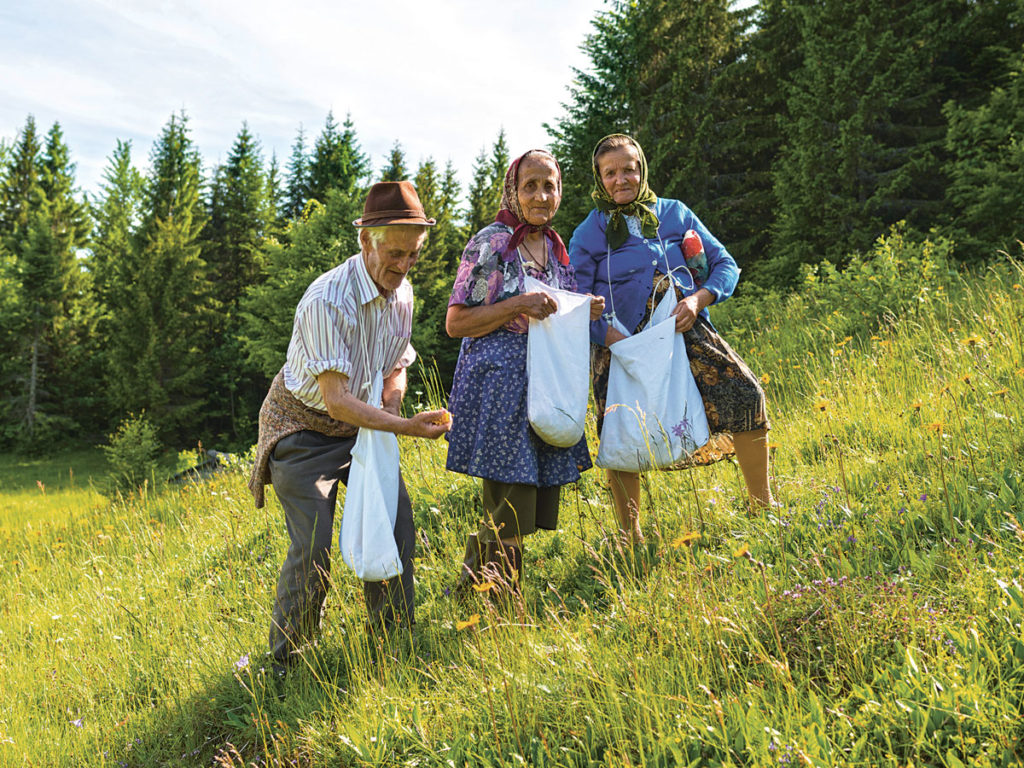
\includegraphics[width=0.8\textwidth,angle=0]{abb/Arnika/Arnikapfluecker-1024x768}
 \caption{ArnikapflückerInnen in den Karparten \citep{Mestrovic2019}}
\label{fig:pfluecker}
\end{figure}

Der Arznei- und Naturkosmetikhersteller Weleda aus Schwäbisch Gmünd setzt, nach ebenfalls vergeblichen Versuchen \textit{Arnica montana} in Deutschland anzubauen, auf nachhaltige Wildsammlungen im Apuseni-Gebirge in Rumänien (Siehe Abbildung~\ref{fig:pfluecker}, S.\pageref{fig:pfluecker}). Das seit 2010 bestehenden rumänischen Unternehmen Bioflora Apuseni führt nachhaltige Wildpflückungen durch und setzt sich dafür ein, dass das Grünland nur durch extensive Viehwirtschaft und ohne jegliche zusätzliche Düngergaben genutzt wird. Die von Hand gepflückten Blüten werden vor Ort in einer von Weleda finanzierten Trocknungsanlage getrocknet. Weleda möchte die Wildsammlungen in weiteren Teilen der Karparten ausdehnen, um auch dort durch Bewirtschaftung die Biodiversität zu erhalten \citep[vgl.][]{Weleda2019}. 

\subsection{Projekt zum Schutz der Biodiversität in Rumänien}

%„schützen durch nutzen“


%Einordnung meiner Arbeit in Relation zum Projekt??? -> Testflüge erwähnen, Zeitrahmen erwähnen???
Das Projekt zum Schutz der Biodiversität in Rumänien ist eine bilaterale Zusammenarbeit im Apuseni-Gebirge zum Erhalt des oligothrophen Grünlandes und insbesondere der Zielart Arnica montana. In zwei Ansätzen soll unter dem Einsatz von moderner Fernerkundungstechnologien einerseits brachliegende Flächen und andererseits Grasland mit Arnica montana erkannt werden. Mit den Erkenntnissen soll auf brachliegenden Probeflächen mit Mäh- und Mulchmaschinen ein Wiesenmanagement stattfinden. Durch die Verwendung von Drohnen sollen bisher unbekannte Flächen mit Arnica montana identifiziert werden, um so mit einer nachhaltigen Arnika-Ernte und Bewirtschaftung die Biodiversität zu erhalten. Das Projekt möchte sich in der Region für Nachhaltigkeit und Naturschutz einsetzten, unter Steigerung des Wohlergehens der lokalen Bevölkerung. 

\subsubsection{Projektpartner}
Das Projekt ist eine Zusammenarbeit der Albert-Ludwigs-Universität Freiburg (ALU-FR) mit dem rumänischen Unternehmen Bioflora Apuseni (BFA) und der Universität für Agrarwissenschaften und Tiermedizin Cluj-Napoca (USAMV). Die ALU-FR wird vertreten durch Prof. Dr. Dr. h.c. Albert Reif (Proffessur für Standort- und Vegetationskunde), Dr. Evelyn Ruşdea  (Projektmanagement) und durch Dr. Holger Weinacker (Institut für Fernerkundung und Landschaftsinformationssysteme). Die ALU-FR hat stellvertretend für das Projekt einen Finanzierungsantrag bei der Deutschen Bundesstiftung Umwelt gestellt.

Das Unternehmen Bioflora Apuseni (BFA) wurde 2010, nach einem langen Prozess der deutsch-rumänischen Zusammenarbeit und Forschung, gegründet. BFA hat es sich zum Ziel gesetzt die ländlichen Bevölkerung im Zentrum des Apuseni Gebirges im nachhaltigen Umgang mit natürlichen Ressourcen zu unterstützten, um die artenreiche Kulturlandschaft der oligotrophen Graslandes zu erhalten und den Lebensstandard zu erhöhen. Das Hauptprodukt ist Arnica montana, welches von den rund 25 SaisonarbeiterInnen von BFA nachhaltig gesammelt und dann in einer lokalen Trocknungsanlage getrocknet. Hauptabnehmer zu einem fairen Preis ist Weleda, die auch gemeinsam mit BFA regelmäßige Schulungen für lokale PflückerInnen organisieren, um die nachhaltige Ernte der Arnikablüten sicherzustellen. Es gibt Entwicklungen? weitere Heilpflanzen zu vermarkten und neue Abnehmer zu finden. Außerdem initiiert BFA weitere Pilotprojekte in anderen Regionen Rumäniens, damit auch dort Arnika nachhaltig geerntet werden kann \citep[vgl.][]{ECOKARST2018,DBU2018}.

Die Universität in Cluj-Napoca (USAMV) erforscht seit 2000 im Apuseni Gebirge die traditionelle Bewirtschaftung des Graslandes, um das Management zu optimieren und zu erhalten. Es gibt unter anderem eine Langzeitstudie zu den Folgen von Düngern auf die Biodiversität des Graslandes im Apuseni Gebirge. Als assoziierter Partner wird der Drohnen-Pilot und Videoeditor Paul Crişan für das Projekt an der USAMV angestellt. Weitere assoziierte Partner sind der Naturpark Apuseni, die LEADER-Initiative (GAL Arieşul Mare) sowie die Firma Weleda.

Bereits von 2000 bis 2004 gab es eine erste Zusammenarbeit der ALU-FR mit der rumänischen USAMV mit dem gemeinsamen „Projekt Apuseni“, aus dem die Identifizierung von Arnica montana im Zentrum des Apuseni Gebirges hervorging. Finanziert durch das Bundesministerium für Bildung und Forschung (BMBF) wurden sieben kleinere Pilotprojekte in verschiedenen Bereichen, wie ländlichem Tourismus, Landwirtschaft, Wasserversorgung, Arzneipflanzen und Waldwirtschaft durchgeführt. Dabei wurde bewusst ein partizipativer Ansatz (buttom-up) gewählt, da vor Ort die Landschaft Allgemeingut ist, das von vielen Menschen beansprucht wird. Deshalb wurden auch möglichst viele Personen in den Prozess der Entwicklung eines nachhaltigen Landschaftmanagements involviert. Neben Interviews mit LandwirtInnen, ExpertInnen und lokalen PolitikerInnen wurden Treffen, Workshops und  Vorträge organisiert, Informationsmaterialien verteilt, Beratungen und Rollenspiel durchgeführt und ein Schul-Projekt „Planning for real“ angeboten. Darin bauten die SchülerInnen gemeinsam ein dreidimensionales Modell des Dorfes, wie es in 15 Jahren aussehen soll. Aus den Projekten ließen sich die Stärken und Schwächen der Bergregion herausfiltern, um damit Empfehlungen für die regionale Entwicklung zu formulieren? \citep[vgl.][]{RUSDEA2009}.
Im Anschluss startete ein weiteres Projekt, diesmal mit dem Schwerpunkt auf \textit{Arnica montana}, 2004 im Apuseni Gebirge. Das „Arnika Projekt“ lief bis 2007 und wurde vom World Wide Fund For Nature (WWF) und der Darwin Foundation is Zusammenarbeit mit der USAMV durchgeführt. Im Ausbau der Kooperation mit der lokalen Bevölkerung wurde der Kontakt zu BesitzerInnen von oligotrophen Wiesen und potenziellen Arnika PflückerInnen hergestellt. Durch Interviews wurde die traditionelle Bewirtschaftung der oligotrophen Wiesen erforscht und Trainings zur nachhaltigen Ernte der Blütenstände der \textit{Arnica montana} durchgeführt \citep[vgl.][20]{DBU2018}.

\begin{figure}[htb]
 \centering
 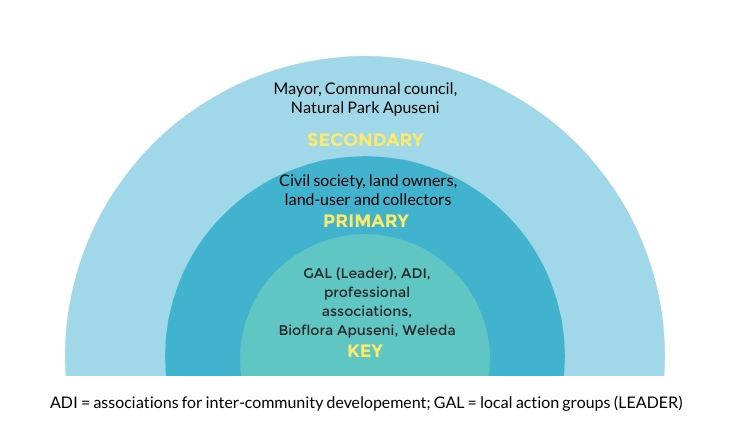
\includegraphics[width=0.7\textwidth,angle=0]{abb/Stakeholder-map}
 \caption{Stakeholder map \citep[In Anlehnung an][]{DBU2018}}
\label{fig:stakeholdermap}
\end{figure}

%Stakeholder map erklären:
Im Projekt wird zwischen Key Stakeholder, primären und sekundären Stakeholdern unterschieden (Siehe Abbildung~\ref{fig:stakeholdermap}, S.\pageref{fig:stakeholdermap}). Die etablierten Organisationen, wie BFA, Weleda und die lokale Aktionsgruppe (LAG/GAL) Arieşul Mare und die Associations for inter-community development (ADI) sind aufgrund von ihrer Erfahrung im Naturschutz vor Ort die Key Stakeholder. Primärer Stakeholder ist die ansässige Bevölkerung, insbesondere die EigentümerInnen oder PächterInnen der Flächen oder SammlerInnen der Wildkräuter. Als sekundäre Stakeholder bilden die die administrativen Stellen in der lokalen und regionalen Behörden und die Verwaltung des Naturparks Apuseni.

\subsubsection{Ökologischer Hintergrund}

Das Apuseni Gebirge befindet sich im nordwestlichen Teil von Siebenbürgen in Rumänien. Es bildet den nördlichen Teil der Rumänischen Westkarpaten und erreicht Gipfelhöhen von 1100 bis 1800 m. Die Landschaft ist geprägt durch Steilhänge und Karstformen, wie Dolinen, Polje, Trockentälern, Karsttreppen und Unterirdischen Höhlen. Die Region hat eine geringe Einwohnerdichte, aber die höchste Einwohnerdichte im Vergleich zu anderen Bergregionen Rumäniens. Vor einer Besiedelung gab es ursprünglich nur Waldgebiet mit Kiefer und Buchen. Durch die Nutzung der Ressource Holz entstand das Grasland von heute. Die Landnutzung beträgt heute noch ca. 55\% Wald (davon ca. 79\% Laubwald, 12,34\% Nadelwald und 3,5\% Mischwald, Rest ist Übergangsvegetation), 17,4\% Grasland, 3,09\% Brachland, 1,84\% Besiedelung und 0,61\% Ackerland (Gärten).

Vor 1989 war die Waldwirtschaft in Rumänien streng geregelt und kontrolliert. In der Zeit danach nahm die Walddegradation und Entwaldung im Apuseni Gebirge stetig zu, weil der kommerzielle Vermarktung von Holz europaweit als wirtschaftlich rentable erkannt wurde. Dies führte zum drastischen Rückgang der Wälder im Apuseni-Gebirge, insbesondere von Nadelbäumen. Die derzeitige Regierung versucht dem entgegen zu wirken und hat neue Regelungen erlassen, nach denen pro Person nur 20m\textsuperscript{3} Holz im Jahr gefällt werden dürfen. Größere Unternehmen sind davon ausgenommen, was einen Nachteil für die lokalen Bevölkerung darstellt, die ihre Haupteinnahmequelle, die Holzverarbeitung und Aufwertung, verliert. Eine signifikante Abwanderung ist die Folge, was auch einen negativen Effekt auf das Management von Grasland hat.

\begin{figure}[htb]
 \centering
  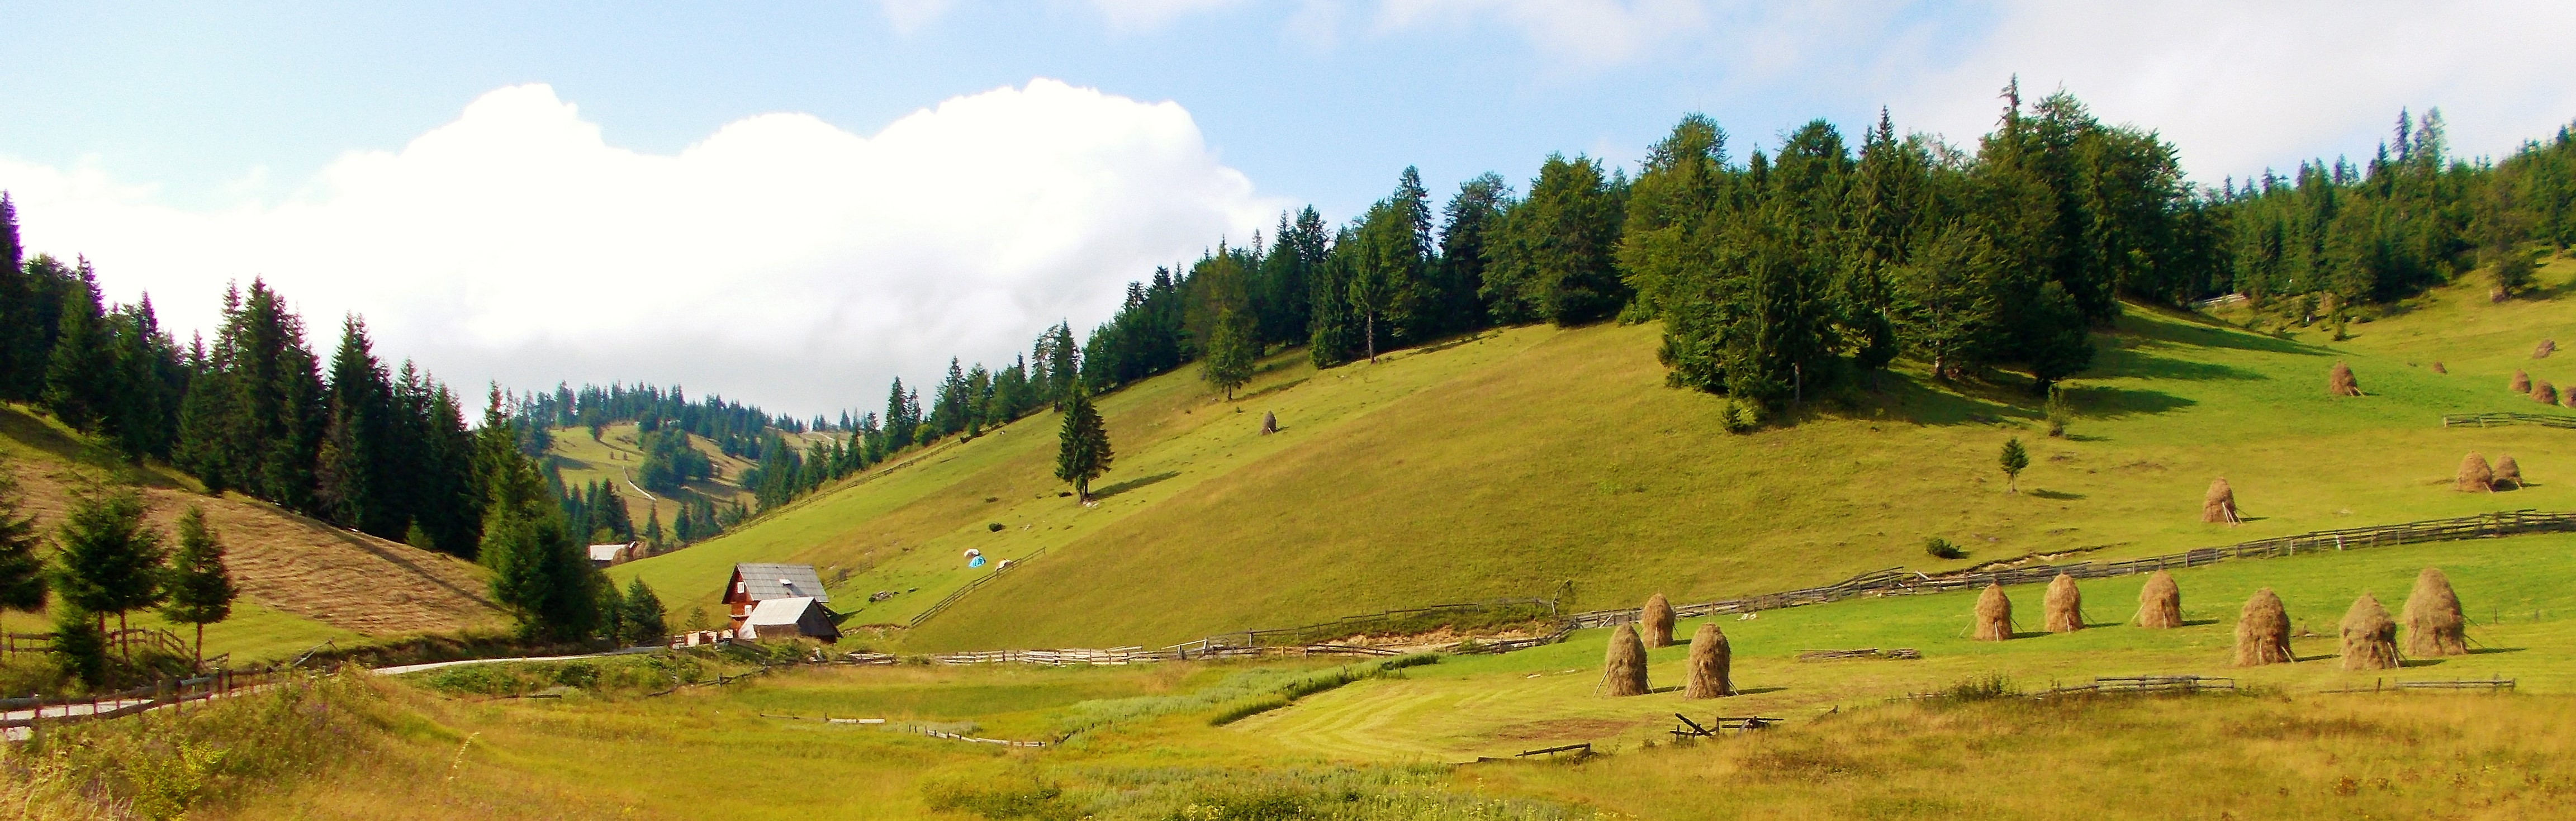
\includegraphics[width=\textwidth,angle=0]{abb/Arnika/apusenimountain2016}
 \caption{Apuseni Gebirge mit traditioneller Heuernte \citep{Farcas2019}}
\label{fig:apuseni}
\end{figure}

Das oligotrophe Grasland kann seine Biodiversität nur erhalten, wenn eine Bewirtschaftung stattfindet. Das Brachliegen oder die Intensivierung der Nutzung gefährdet das schwierige Gleichgewicht der Graslandwiesen. Zum Schutz der Biodiversität muss eine gemäßigte Düngung von biologischen Düngern (keine Mineraldüngung!) periodisch aufgetragen werden. Um optimale Bedingungen für eine hohe Vielfalt an Arznei- und Wildpflanzen zu erhalten, müssen die Flächen etwa jährlich gemäht werden und dazwischen geflegt werden, z.B. durch das Entfernen von Ästen und Steinen.

\tg{hier muss noch zu dem tatsächlichen Manangement recherchiert werden}

\subsubsection{Vorgehensweise}

Der Projektzeitplan sieht einen Start ab dem Frühjahr 2019 vor und das Projekt soll über einen Zeitraum von drei Jahren laufen. Jährlich im Juni/Juli sollen die Drohnenflüge zur Identifizierung von Arnika stattfinden. Im September/Oktober werden die Grasland-Flächen beflogen, um eine Bewirtschaftung oder das brachliegen festzustellen. Zur Vorbereitung auf die Datenerhebungen in Rumänien fanden im Juli 2018 Drohnenflüge zu Testzwecken im Schwarzwald statt.

Zur Identifikation von brachliegendem oligotrophen Grasland sollen mit dem Einsatz von Drohnen Digitale Höhenmodelle erstellt werden. Dafür muss das gesamte Gelände zweimal mit der Drohne erfasst werden. Beim ersten Flug wird ein Digitales Oberflächen Modell (DOM) (engl. digital surface model DSM) erstellt, also ein Modell der Erdoberfläche inklusive auf ihr befindlicher Objekte, wie die Vegetation. Nach dem zweiten Flug kann ein Digitales Geländemodell (DGM) (engl. digital terrain model DTM) abgeleitet werden. Das DGM ist ein Modell der natürlichen Erdoberfläche ohne Objekte. Durch die Subtraktion der beiden Modelle kann ermittelt werden, ob Flächen gemäht wurden oder ob sie brachliegen. Nach der Indentifikation von brachliegenden Flächen werden fünf Probeflächen in fünf Gemeinden ausgewählt und durch den Einsatz von Mäh- und Mulchmaschinen wieder nutzbar gemacht. In Zusammenarbeit mit der lokalen Aktionsgruppe Arieşul Mare soll der Kontakt zwischen LandbesitzerInnen initiiert werden. Mit dem Zusammenschluss gibt es die Perspektive weitere Technologien und Maschinen anschaffen zu können und das Projekt auf andere Regionen ausweiten zu können.

Mit der nachhaltigen Vermarktung von Arnica montana soll in die Bevölkerung ein Interesse zum Schutz des oligotrophen Graslandes geschaffen werden. Durch die Verknüpfung der ökonomischen Interessen mit dem ökologischen Erhalt der Biodiversität soll langfristig eine Steigerung der Lebensqualität der vor Ort lebenden Menschen erreicht werden. An die Entwicklung der BFA soll hier angeschlossen werden. Ziel ist es eine Datenbank und Karte über die Verteilung der Arnika-Flächen in zehn Gemeinden zu erstellen. Durch den Einsatz von Drohnen in fünf Gemeinden soll das Produktivitätspotential der Habitate ermittelt und in eine qualitative Klasse in Abhängigkeit von der Anzahl der Blütenstände pro 100 m\textsuperscript{2} eingeordnet werden. Zusätzlich soll erfasst werden, welches Management bisher auf den Flächen durchgeführt wurde. Für die Auswertung der durch den Drohneneinsatz entstandenen Bilder soll ein Software-Programm entwickelt werden, dass die Arnica montana Blütenstände automatisch erkennt und eine Klassifizierung durchführt.

\subsection{Drohneneinsatz zur Fernerkundung}

%+++ Was ist eine Drohne? Was eine UAS, UAV?
Drohnen sind Luftfahrzeuge\fio{test, hier kommt mal ein längerer test satz und wie er so dargestellt wird.}, die ohne an Bord befindliche Personen über einen Computer oder vom Boden aus über eine Fernsteuerung betrieben werden. Unbemannte Luftfahrzeuge (engl. Unmanned Aerial Vehicle, kurz UAV) besitzen zwei Tragflächen und sind dem Flugzeug nachempfunden. Multikopter zählen zu den Hubschraubern und haben zwischen zwei und zwölf Rotoren, so können sie sich in alle Richtungen bewegen. Beide werden im allgemeinen Sprachgebrauch Drohnen genannt. Ferngesteuerte Fluggeräte, die im Freizeitbereich eingesetzt werden, zählen nicht zu den Drohnen, auch wenn vor allem die Multikopter Flugmodelle oft so bezeichnet werden. Unmanned Aerial Systems (UAS) bestehen aus der UAV, der Sensor-Ladung und der Bodenkontrollstation. Komponenten und Größe der Bodenkontrollstationen variieren stark, in Abhängigkeit von der Aufgabe der UAV. Sie können aus großen Kontrollsystemen bestehen, die auf Fahrzeugen montiert werden oder nur aus einem kleinen Laptop, der getragen werden kann. Die Klassifizierung von UAS im zivilen wissenschaftlichen Einsatz orientiert sich generell auf den schon vorhandenen militärischen Begriffen. Die Einteilung basiert auf den Eigenschaften Größe, Flugausdauer und weiteren Fähigkeiten der Drohnen \citep[vgl.][]{Watts2012}.

\subsubsection{Vergleich von Drohnenarten}

Für den Anwendungsmaßstab des Projekts in Rumänien sind zwei Arten von Drohnen geeignet (Siehe Abbildung~\ref{fig:drohnen}, S.\pageref{fig:drohnen}). Die Multikopterdrohnen können präzise Aufnahmen in einer angemessene Höhe machen, haben durch den Schwebflug aber einen höheren Energieverbrauch und somit eine kürzere Flugdauer. „Vertical Take-Off and Landing“ (VTOL) Drohnen sind UAV, die keine Start- oder Landebahn benötigen. Durch ihre Tragfläche können VTOL Drohnen eine große Fläche in geringer Zeit befliegen. Zum Starten und Laden haben sie Rotoren, die nach oben gerichtet werden. Dadurch sind sie auch in unwegsamen Gelände einsetzbar.
Generell stehen die mögliche Flugzeit und damit auch die Größe der Fläche, die von der Drohne erfasst werden kann, in Abhängigkeit zum Gewicht der Drohne. Eine höhere Beladung, durch weitere Sensoren, beispielsweise eine Kamera mit einem größerem und schwerem Objektiv, bringen genauere Ergebnisse, aber verkürzen durch ihr Gewicht die mögliche Flugzeit. Einen großen Teil des Gewichts macht aber auch der Akku aus, dessen Größe sich aber auch positiv auf die Flugdauer auswirkt.

\begin{figure}[hbt]
    %\hspace{-20pt}
    \subfigure{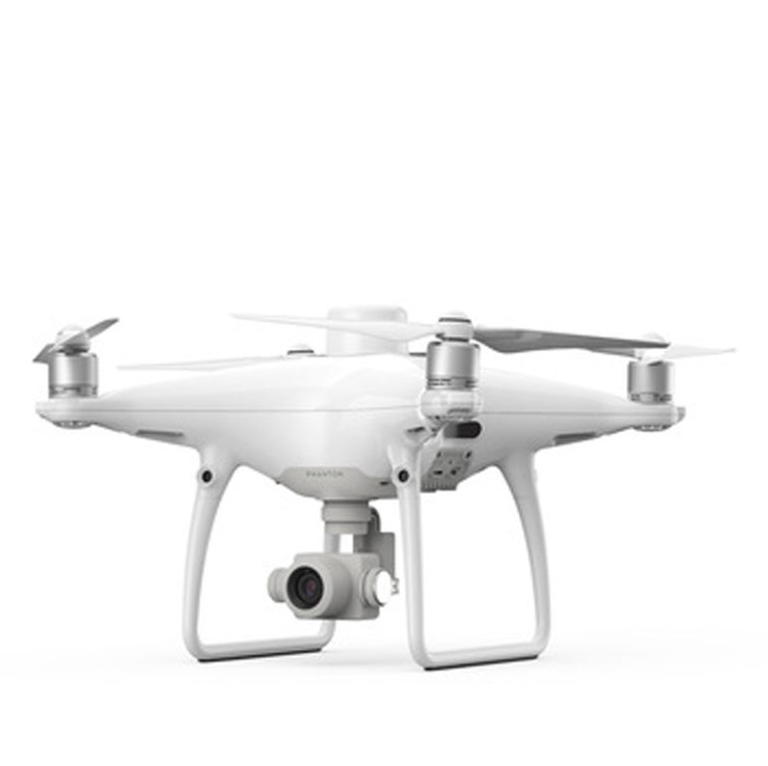
\includegraphics[width=0.20\textwidth]{abb/drohnen/P4RTK}}
    \hspace{-20pt}
    \subfigure{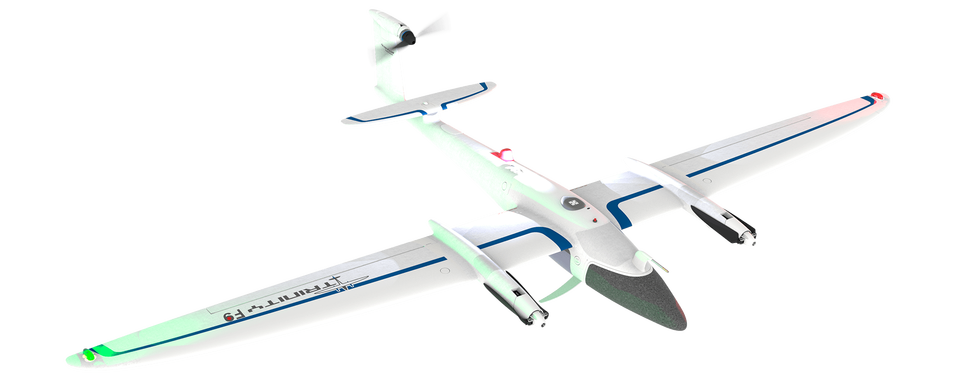
\includegraphics[width=0.52\textwidth]{abb/drohnen/trinity-f9}}
        \hspace{-30pt}
    \subfigure{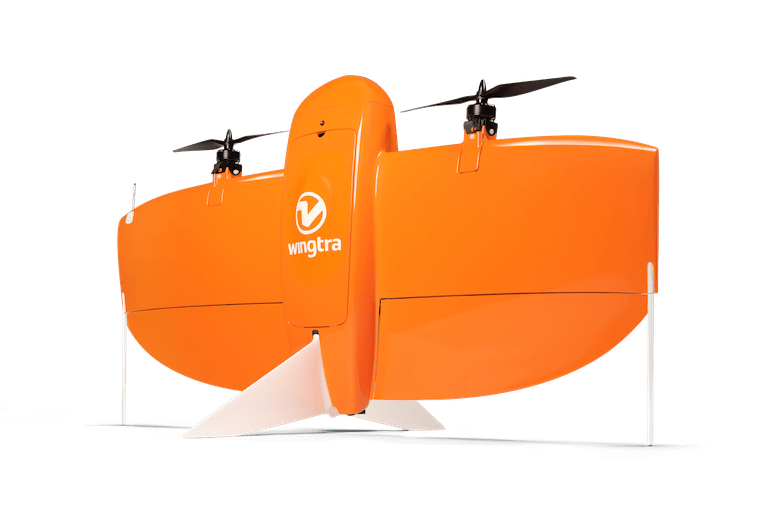
\includegraphics[width=0.35\textwidth]{abb/drohnen/wingtraone}}
     \hspace{-20pt}
\caption{ v.l.n.r: DJI Phantom 4 Quadrocopter \citep{DJI2019}, Trinity F9 \citep{QSGH2019} und WintraOne VTOL-Drohnen \citep{Wingtra2019}}
     \hspace{-40pt}
  \label{fig:drohnen}
\end{figure}

Das „Projekt zum Schutz der Biodiversität in Rumänien“ behandelt zwei Aufgaben, die unterschiedliche Anforderungen an eine Drohne stellen. Bei der Befliegung des Graslandes zur Erkennung von brachliegenden Flächen ist eine riesige Fläche zu erfassen. Eine UAV mit Starrflügeln kann im Vergleich zu Multikoptern höher fliegen und hat somit eine größere Flugausdauer, so kann eine größere Fläche abdeckt werden. Mit einer „Vertical Take Off and Landing“ Drohne (VTOL) können Schäden beim Start oder Ladung in unebenen Gelände vermieden werden. Da die Vegetation des Graslandes nur eine Höhe von 20-30 cm hat, muss zur genauen Berechnung der Höhenmodelle die möglichst genaue vertikale und horizontale Position der Drohne erfasst werden. Dementsprechend wird ein System  benötigt, dass die Ungenauigkeiten der globalen Navigationssysteme (GNSS), die üblicherweise ein paar Meter betragen, ausgleicht. Mit real-time kinematics (RTK) und post-processing kinematics (PPK) Systemen kann eine genaue Positionsbestimmung bis auf wenige Zentimeter berechnet werden. Wie der Name schon sagt, findet diese Berechnung beim RTK in unmittelbar statt, beim PPK nachgelagert. 
Der Vorteil von RTK und PPK ist, dass die Verwendung von Bodenreferenzpunkten entfällt, was Kosten spart. Für Beide wird eine GNSS-Bodenstation benötigt, die georeferenziert ist, um ein genaues Ergebnis zu erzielen. Bei PPK kann auch falls vorhanden mit einer virtuellen Referenzstation gearbeitet werden. Bei RTK muss eine Verbindung zwischen Drohne und GNSS-Bodenstation vorhanden sein, bei Störungen kann ein genaues Ergebnis nicht berechnet werden. Bei PPK ist eine Verbindung nicht notwendig, die genaue Positionierung wird erst bei Auswertung der Log-Daten berechnet. 

Für die Identifizierung von 5-8 cm großen Arnika-Blüten benötigt man hingegen eine Drohne, die Bilder in einer möglichst hohen Auflösung machen kann. Da Starrflügel UAVs eine höhere Mindestgeschwindigkeit haben als Multikopter, die auch in der Luft „stehen“ können, könnte sich die Fluggeschwindigkeit negativ auf die Qualität der Bilder auswirken. Einerseits sollen großflächige Befliegungen Flächen mit Arnica montana lokalisieren, um das Monitoring auszuweiten. Andererseits soll eine qualitative Analyse der Flächen stattfinden. Für die großflächige Befliegung eignet sich eine VTOL-Drohne, die eine möglichst hohe Auflösung erzielt dabei aber eine große Fläche befliegen kann. Für die qualitative Analyse der Flächen kann noch höhere Auflösung nötig sein, die durch eine tiefere Flughöhe mit geringer Geschwindigkeit erreicht werden. Mit einem Multikopter kann dies ohne große Umstände passieren.

\begin{table}[hbt]
\fontfamily{cmss}\selectfont
\footnotesize
\begin{tabular}{lccc} %\toprule
\textbf{Technische Daten} & \textbf{DJI Phantom 4 RTK} & \textbf{Trinity F9}  & \textbf{WingtraOne} \\ %\midrule
\hline\hline
Flügelbreite & 0,35 m & 2,394 m & 1,25 m \\
Max. Startgewicht & 1,391 kg & 4,5 kg & 4,5 kg \\
max. Zuladung & – & 550 g & 800 g \\
Fluggeschwindigkeit & max 50 – 58 km/h & 60 km/h & 57,6 km/h \\
Max. Flugzeit & 30 min & 60 min & 55 min \\
Windwiderstand am Boden & 10 m/s & 7 m/s & 8 m/s \\
Windwiderstand im Flug & 10 m/s & 12 m/s & 12 m/s \\
Max. Fläche & 100 ha (182 m) & 500 ha (100 m) & 320 ha (120 m) \\
Auflösung & 1,5 cm/px (120 m) & 2,5 cm/px (100 m) & 2,8 cm/px (120 m) \\
Sensoren & RTK und Gimbal\textsuperscript{1} & PKK & PKK \\
Positionierungsgenauigkeit\textsuperscript{2} &  & 2 – 5 cm &  \\
{    } vertikal & 1,5 cm + 1 ppm RMS &  & 2 cm  \\
{    } horizontal & 1 cm + 1 ppm RMS &  & 1 cm + 0,003\% RMS\\
Preis & ca. 7.800 EUR & ca. 14.850 EUR & ca. 36.678 EUR\\
\hline
\end{tabular}
\\
\scriptsize
1: Gimbal ist ein Bildstabilisator \\
2: RMS = Root Mean Square entspricht der Standardabweichung \\
1 ppm = pro km nimmt Wertgenauigkeit um 1 mm ab. 
\caption{Technische Daten der Drohnen im Vergleich \citep[vgl.][]{DJI2019,QSGH2019,Wingtra2019}}
\label{tab:technischedaten}
\end{table}

Derzeit gibt es eine Vielzahl von Drohnen in allen Preissegmenten zum privaten und wissenschaftlichen Gebrauch auf dem Markt. Drei Vertreter, die für die Aufgaben des Projektes in Rumänien in Frage kommen würden, sind der Quadrocopter DJI Phantom 4 RTK, die VTOL-Drohne Trinity F9 von Quantum-Systems und die VTOL-Drohne WintraOne PPK. Ausgewählt wurden diese weil sie alle ein System zur Positionskorrektur (PPK oder RTK) besitzen. Dies ist notwendig, um genaue digitale Höhenmodelle zu berechnen. Schaut man sich die drei Drohnen an (Siehe Abbildung~\ref{fig:drohnen}, S.\pageref{fig:drohnen}), fallen zunächst die großen äußeren Unterschiede auf. Mit einer Flügelbreite von über 2 m ist die Trinity F9 die größte Drohne. Die WingtraOne ist für eine Starrflügel Drohne mit einer Flügelbreite von nur 1,25 m recht klein. Trotzdem sind beide VTOL-Drohnen, können also aus dem Stand starten. Die Trinity F9 dreht dafür ihre Rotoren nach oben und schwebt waagerecht in die Luft, vergleichbar mit einem Multikopter. Die WintraOne starten senkrecht in die Luft und dreht dann in gewünschter Höhe den Flugkörper. Vergleicht man die Technischen Daten der Drohnen (Siehe Tabelle~\ref{tab:technischedaten}, S.\pageref{tab:technischedaten}) unterscheiden sie sich im Windwiderstand, also die maximale Windgeschwindigkeit bei der mit den Drohnen geflogen werden sollte, nur geringfügig. Auch bei der Fluggeschwindigkeit scheint es nur minimale Unterschiede zu geben, allerdings ist dies bei der DJI Phantom 4 RTK die maximale Fluggeschwindigkeit, der Quadrocopter kann durchaus auch wesentlich langsamer fliegen und damit genauere Bilder aufnehmen. Bei den VTOL-Drohnen ist die angegebene Fluggeschwindigkeit die „cruise speed“ also durchschnittliche Fluggeschwindigkeit im aerodynamischen Flug, ein wesentlich geringere Fluggeschwindigkeit ist nicht möglich. Der Quadrocopter unterscheidet sich im Vergleich zu den beiden VTOL-Drohnen wesentlich in Größe, Gewicht und Zuladungsmöglichkeit. Die DJI Phantom 4 RTK Drohne wiegt nur 1391 g Größe von nur 35 cm in der Diagonale. Eine zusätzliche Zuladung ist nicht möglich, die Kamera und Sensoren sind integriert. Trotz des wesentlich geringerem Gewichts der Drohne kann sie nur etwa 30 min fliegen und damit etwa halb so lang, wie die VTOL-Drohnen. Die Fläche die von der Drohne erfasst werden kann, ist dementsprechend auch wesentlich geringer, nur 100 ha bei einer Flughöhe von 182 m. Mit der WingtraOne Drohne kann eine Fläche von 320 ha bei 120 m Flughöhe erfasst werden, mit der Trinity F9 sogar 500 ha bei 100 m Flughöhe. Allerdings haben die Bilder, die bei der Flughöhe von den VTOL-Drohnen gemacht werden nur eine Auflösung von 2,5 cm/px (Trinity F9 bei 100 m) bis 2,8 cm/px (WingtraOne bei 120m). Die DJI Phantom 4 RTK schafft bei 120 m Flughöhe eine deutlich bessere Auflösung mit 1,5 cm/px. Ein weiterer entscheidener Unterschied besteht in der Positionierungsgenauigkeit. Die DJI Phantom 4 RTK und die WingtraOne PKK erreichen eine Genauigkeit von etwa 1 bis 2 cm. Die Trinity F9 erreicht mit ihrem PKK System nur eine Positionsgenauigkeit von 2 bis 5 cm. Dies ist, neben dem Preis, der entscheidenste Unterschied zwischen den beiden VTOL-Drohnen WingtraOne und Trinity F9. Preislich ist der Quadrocopter am günstigsten mit 7800 Euro. Die Trinity F9 Drohne ist für etwa 14850 Euro erhältlich und die WingtraOne kostet 36678 Euro. %-> Ein Vorteil der DJI Phantom 4 RTK ist auch noch das Ausweichsystem, ???
Für die Aufgabe der Erfassung von brachliegenden Flächen im „Projekts zum Schutz der Biodiversität in Rumänien“ sind die Trinity F9 und die WingtraOne Drohne geeignet. Allerdings können bei der Berechnung der digitalen Höhenmodelle mit der Trinity F9 aufgrund von der geringeren Positionierungsgenauigkeit Fehler entstehen. Die WingtraOne hat dort einen entscheidenen Vorteil. Für die Erkennung von Arnica montana könnte mit einer VTOL-Drohne ein größeres Gelände beflogen werden, um einen Hinweis auf Arnica montana zu geben, für eine präzise qualitative Analyse könnten mit der DJI Phantom 4 RTK gute Ergebnisse erzielt werden. Eine Drohne, die für beide Aufgaben mit besten Ergebnissen verwendet werden kann, ist die WingtraOne. Mit einer geringen Flughöhe und einer lichtempfindlichen Kamera kann auch die WingtraOne Bilder mit einer Auflösung machen, die eine qualitative Analyse von Arnikablüten möglich macht. 

\subsubsection{Testflüge im Schwarzwald}
%++++++ Testflüge?? im Schwarzwald 

Bei Testflügen im Schwarzwald im Juli 2018 wurden erste Bilder an einem bekannten Standort von Arnica montana gemacht. Mit der Octocopter-Drohne der Universität Freiburg wurden mit einer Sony Alpha 7R Kamera eine Fläche in unterschiedlichen Flughöhen erfasst. 
\begin{wrapfigure}{r}{0.4\textwidth}
  \vspace{-30pt}
  \begin{center}
    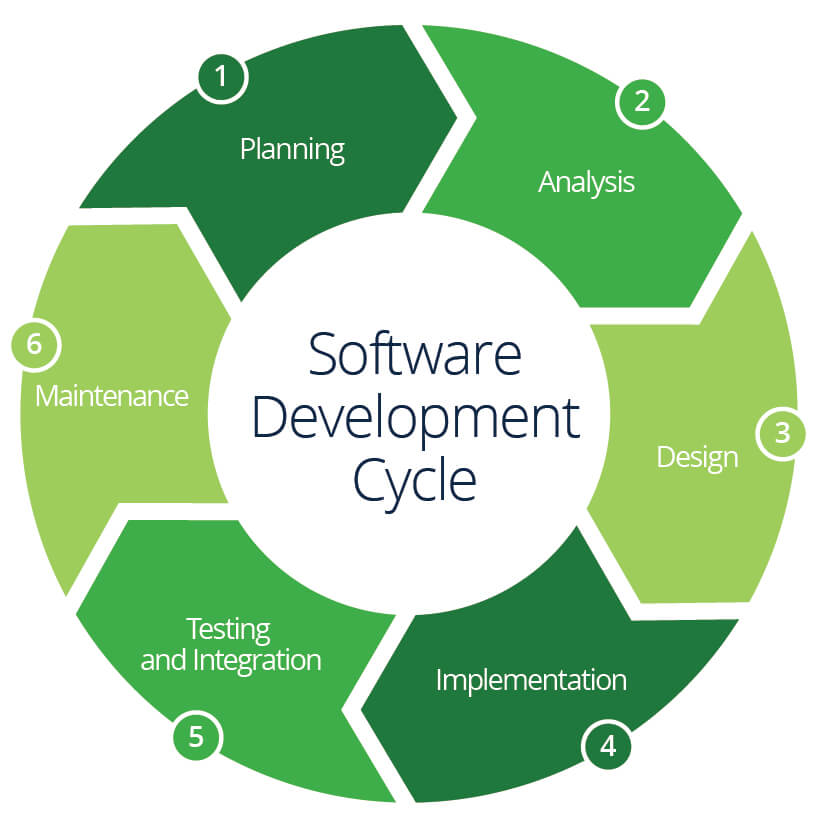
\includegraphics[width=0.4\textwidth]{abb/SDLC}
  \end{center}
  \vspace{-20pt}
  \caption[System Developement Life Circle \citep{Smartsheet2019}]{\footnotesize SDLC \citep{Smartsheet2019}}
  \label{fig:sdlc}
  \vspace{-30pt}
\end{wrapfigure}

Anschließend wurden die Daten ausgewertet, Höhenmodelle berechnet und Orthofotos erstellt. Ziel war es mit den Testflügen den Bedarf und Beschaffenheit der Ausrüstung für die spezifische Aufgabe heraus zu finden. Mit den entstandenen Testdaten sollen erste Methoden? entwickelt werden und damit der System Developement Life Circle (SDLC) in Gang gesetzt (Siehe Abbildung~\ref{fig:sdlc}, S.\pageref{fig:sdlc}). Die Softwareentwicklung durchläuft verschiedene Phasen, die aufeinander aufbauen. Im Laufe der Entwicklung können sich die Phasen im Kreislauf wiederholen, um Änderungen einzuarbeiten und Fehler auszubessern. 


%- die Testflüge dienten als erste Orientierung, um sich darauf vorbereiten zu können, heraus zu finden welches Equipment notwendig ist und mit den entstandenen Bildern die Softwareentwicklung anzustoßen, aber das ist ein langer Prozess, bis dies tatsächlich beeendet ist.

%Ich nehme mir jetzt diese Testdaten und teste wie mit "einfachen" mitteln das erreicht werden kann. 
% - Meine Software bietet die Möglichkeit sich einen Überblick zu verschaffen, für die qualitative Analyse nicht so geeignet.

\begin{table}[hbt]
\fontfamily{cmss}\selectfont
\begin{tabular}{lcccc} %\toprule
\textbf{} & \textbf{Flug 1} & \textbf{Flug 2}  & \textbf{Flug 3} & \textbf{Flug 4} \\ %\midrule
\hline\hline
Flughöhe & 13,8 m & 20,3 m & 27,8 m & 64,6 m \\
Anzahl Bilder & 236 & 208 & 233 & 355 \\
Auflösung am Boden & 1,32 mm/px & 1,89 mm/px & 2,6 mm/px & 5,93 mm/px \\
Erfasste Fläche & 1.04e+03 m\textsuperscript{2} & 633 m\textsuperscript{2} & 950 m\textsuperscript{2} & 0.0174 km\textsuperscript{2} \\
\hline
\end{tabular}
\caption{Technische Daten? der Testflüge}
\label{tab:flugvergleich}
\end{table}

Die vier Flüge sollten in der Höhe von 15 m, 20 m, 30 m und 80 m Aufnahmen machen, um Bilder mit unterschiedlicher Auflösung für die Softwareentwicklung zu haben. Die tatsächliche Flughöhen lassen sich der Tabelle~\ref{tab:flugvergleich} auf S.\pageref{tab:flugvergleich} entnehmen. Gerade beim letzten Flug, weicht die tatsächliche Flughöhe erheblich von der geplanten ab. Auch die Lichtverhältnisse sind bei Flügen sehr unterschiedlich und deutlich auf den Aufnahmen erkennbar (Siehe Abbildung~\ref{fig:gleicheblumen} und \ref{fig:gleicherausschnitt}, S.\pageref{fig:gleicheblumen}. Bei den ersten beiden Flügen in etwa 15 m und 20 m sind die Blüten noch sehr gut erkennbar. Bei den Aufnahmen aus ca. 30 m und 80 m (tatsächlich etwa 65 m) Flughöhe wird die Bildqualität zunehmend schlechter. Die Auflösung beträgt bei 65 m Höhe auf dem Boden nur noch etwa 0,6 cm/px. Das Bild ist sehr unscharf und die Blumen sind nur noch als gelbe Punkte erkennbar. 

\begin{figure}[htb]
    \subfigure[Flug 1]{\includegraphics[width=0.24\textwidth]{abb/ergebnisse/gleicherausschnitt/DSC01525-a}}
    \subfigure[Flug 2]{\includegraphics[width=0.24\textwidth]{abb/ergebnisse/gleicherausschnitt/DSC01298-a}}
    \subfigure[Flug 3]{\includegraphics[width=0.24\textwidth]{abb/ergebnisse/gleicherausschnitt/DSC01757-a}}
    \subfigure[Flug 4]{\includegraphics[width=0.24\textwidth]{abb/ergebnisse/gleicherausschnitt/DSC01959-a}}
\caption{Gleicher Ausschnitt von 2168px bei unterschiedlicher Flughöhe}
  \label{fig:gleicherausschnitt}
\end{figure}

\begin{figure}[htb]
    \subfigure[Flug 1]{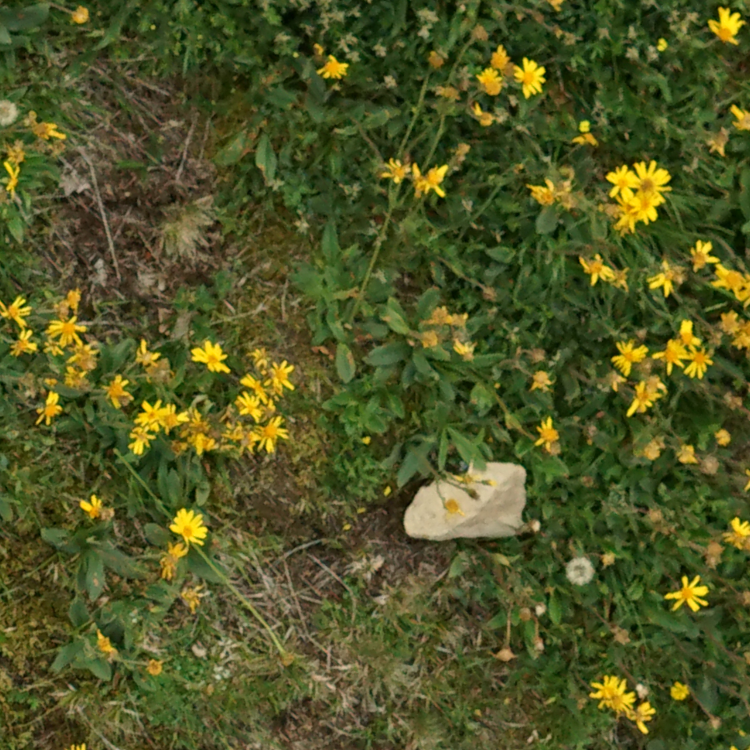
\includegraphics[width=0.24\textwidth]{abb/ergebnisse/gleicheblumen/DSC01525-b}}
    \subfigure[Flug 2]{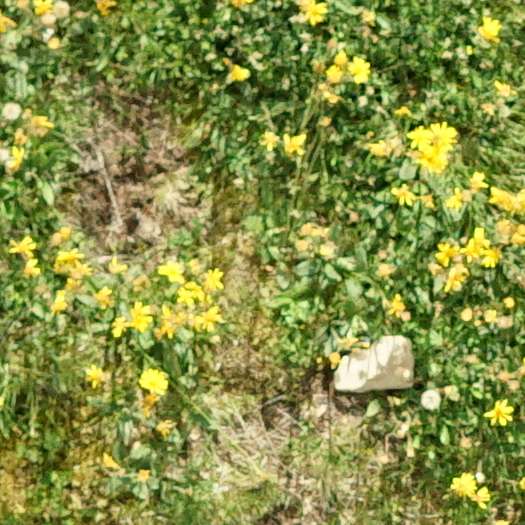
\includegraphics[width=0.24\textwidth]{abb/ergebnisse/gleicheblumen/DSC01298-b}}
    \subfigure[Flug 3]{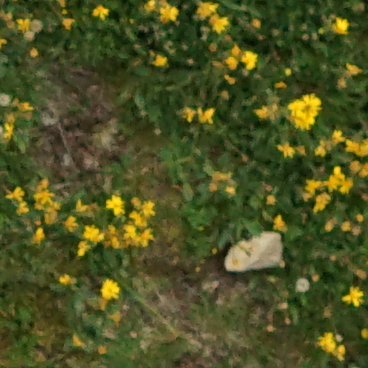
\includegraphics[width=0.24\textwidth]{abb/ergebnisse/gleicheblumen/DSC01757-b}}
    \subfigure[Flug 4]{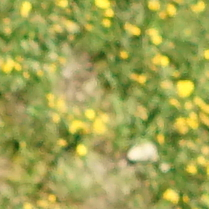
\includegraphics[width=0.24\textwidth]{abb/ergebnisse/gleicheblumen/DSC01959-b}}
\caption{Gleicher Bildausschnitt mit unterschiedlicher Auflösung je nach Flughöhe.}
  \label{fig:gleicheblumen}
\end{figure}

% Testdaten sind Grundlage für mich zur Entwicklung des Programms und zur Bewertung der Funktion, 

% Aufnahmenqualität bewerten
  %- unterschiedliche Lichtverhältnisse der Aufnahmen, Sonnenschein oder Schattenwurf 
  %- durch Bewegung unschärfe, vielleicht auch Belichtungszeit der Kamera nicht gut eingestellt?
  %- 
\blindtext

%   FLUGPLANUNG ??? UND ÜBERLAPPUNG DER BILDER -> ORTHOFOTO?

%++++++++++ wissenschaftlicher Kenntnissstand von Monitoring via Drohnen bzw. von automatischer Erkennung und Programmierung ???

\newpage
\section{Programmbeschreibung}\label{programm}

% Problemstellung/Fragestellung:
Die Anwendungssoftware „Flower Segmentation Tool“ wurde zur Erkennung von Arnica montana durch die Auswertung von Drohnenluftbildern entwickelt. Ziel ist es das Monitoring von Arnica montana durch eine nachhaltige Pflückung auf bisher nicht genutzte Flächen auszuweiten. Durch den Drohneneinsatz können auch in unwegsamen Gelände Erkenntnisse über den Bestand von Arnika gewonnen werden. Als Datengrundlage bei der Entwicklung dienten die Aufnahmen der Testflüge aus dem Schwarzwald des „Projekt zum Schutz der Biodiversität in Rumänien“.
Das „Flower Segmentation Tool“ ist so konzipiert, dass schnelle Berechnungen Aussagen über den Bestand getroffen werden können, die dann vor Ort weiter untersucht werden. Es soll also unterstützend zur Feldarbeit wirken und dabei eine Einschätzung liefern, wo diese stattfinden kann. 
%Anforderungen an den Code
Die wichtigste Anforderung an das Programm ist dabei trotz großer Datenmengen noch in angemessener Schnelligkeit zu agieren. Um eine einfache Installation zu ermöglichen, wurde darauf geachtet niedrigschwellige Soft- und Hardwarevoraussetzungen zu fordern. 
%Anforderungen an die Benutzeroberfläche

\begin{figure}[hbt]
 \centering
 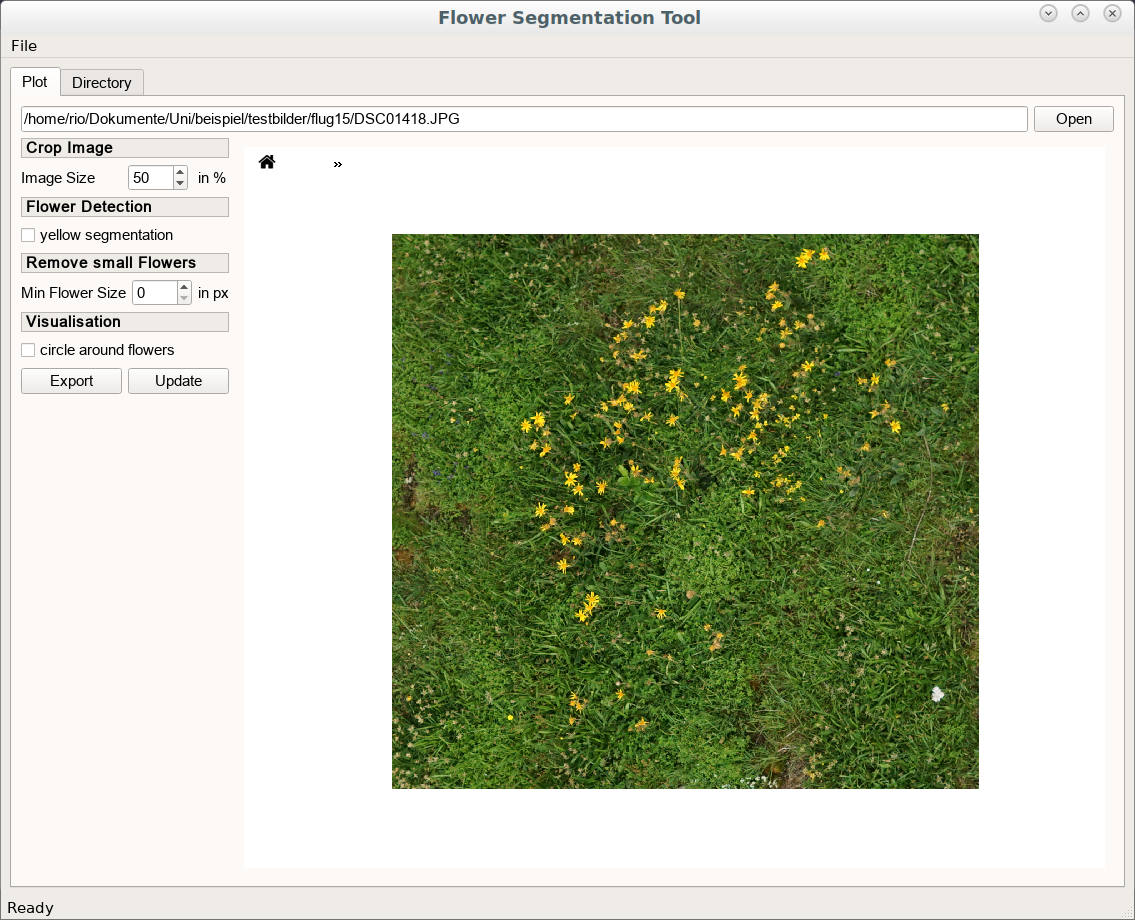
\includegraphics[width=\textwidth,angle=0]{abb/gui/plot-fenster-mit}
 \caption{Grafische Oberfläche mit Plotfenster}
\label{fig:gui-plot}
\end{figure}

Die Grafische Benutzeroberfläche besteht aus zwei Teilen. Einerseits soll die grafische Darstellung der Bilder zum Ausprobieren der Parameter möglich sein (Siehe Abbildung~\ref{fig:gui-plot}, S.~\pageref{fig:gui-plot}). Dabei ist ein vielseitiger Plotfenster mit der Möglichkeit den Ausschnitt zu verändern und Teile des Bildes zu vergrößern eine wichtige Funktion. Andererseits soll eine einfache Anwendung der Berechnung auf einen großen Datensatz möglich sein. Deshalb gibt es unter dem Tab „Directory“ die Eingabe oder Auswahl eines Ordners (Input-Directory), aus dem alle Bilddateien bearbeitet werden (Siehe Abbildung~\ref{fig:gui-dir}, S.~\pageref{fig:gui-dir}). Bei beiden Tabs verschafft eine Statusanzeige im unteren Rand des Anwendungsfensters einen Überblick, welche Prozesse im Hintergrund laufen.

\begin{figure}[htb]
 \centering
 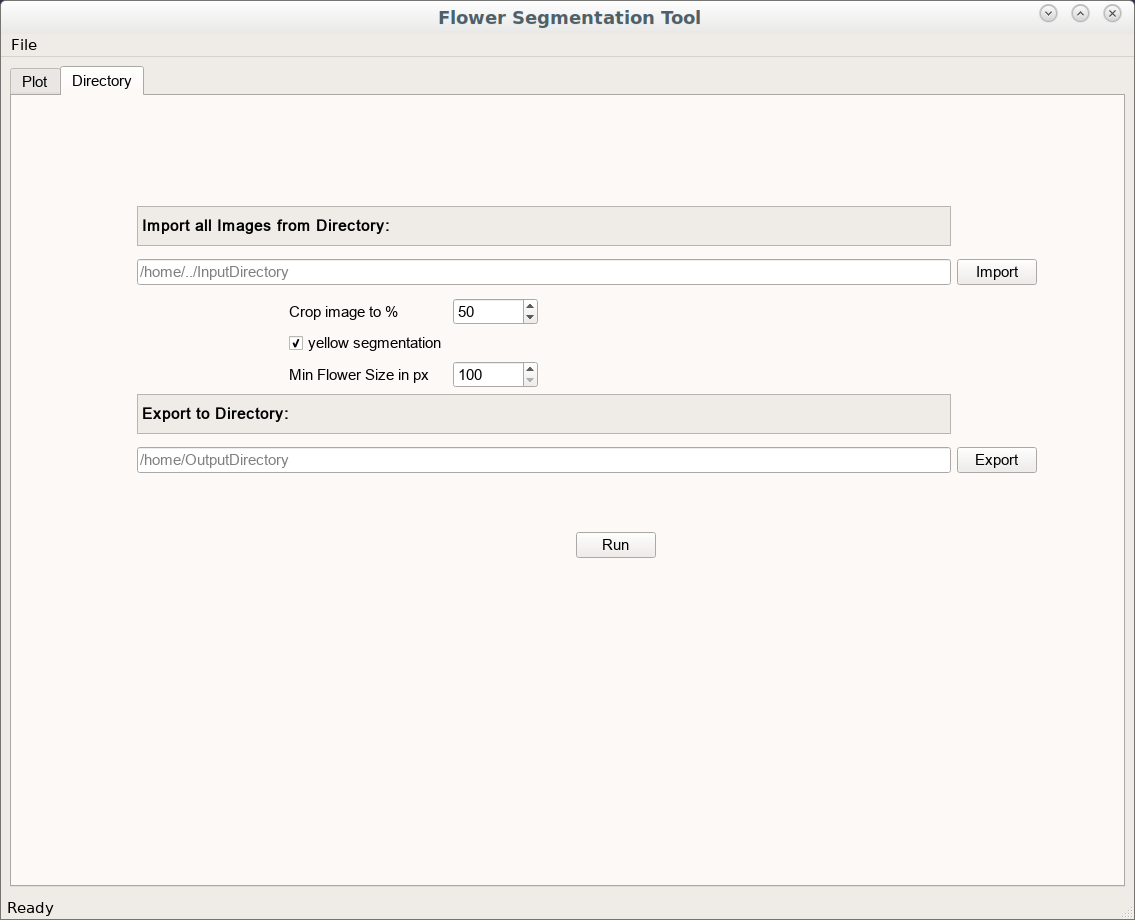
\includegraphics[width=\textwidth,angle=0]{abb/gui/directory-fenster}
 \caption{Grafische Oberfläche zur Anwendung auf Ordner}
\label{fig:gui-dir}
\end{figure}


\subsection{Programmiersprache}
Python ist eine Open Source Programmiersprache, die plattformübergreifend auf allen gängigen Betriebssystemen anwendbar ist. Die interpretierte Skriptsprache wurde 1994 von dem niederländischen Programmierer Guido Rossum als Python 1.0 veröffentlicht. Der Name Python hat Rossum von der britischen Komikergruppe Monty Python abgeleitet.
Entscheidener Unterschied zu anderen höheren Programmiersprachen, ist der gut lesbare und knapp gehaltene Stil von Python. Ziel ist es Redundanz zu vermeiden und Übersichtlichkeit zu optimieren. Zur Strukturierung verwendet Python Einrückungen und kommt mit wenigen Schlüsselwörtern aus. Mit diesem reduzierten Syntax schafft Python Einfachheit, ohne dabei eine Komplexität zu verhindern. Python unterstützt objektorientierte und funktionale Programmierung. Es gibt eine umfassende  Standartbibliothek und zusätzlich die Möglichkeit der Erweiterung einer Vielzahl an Modulen, die in den Skripten import werden können.
%Vielzahl von NutzerInnen (kommerziell, wissenschaftlich, Betriebssystemen, Webframeworks)

%- Python-Interpreter, die stärksten sind CPython, basiert auf der Programmiersprache C und Jython basierend auf Java. 
%-  Compiler, die Python in andere Programmiersprachen übersetzten und dort nutzbar machen.

Seit 2001 wird Python durch die Python Software Foundation stetig weiterentwickelt. 
Python 2 gibt es seit 2000, Python 3 seit 2008. Dies beinhaltet so tiefgreifende Änderungen, dass einige Funktionen, die unter Python 2 geschrieben wurden, nicht mehr unter Python 3 funktionieren würden. Deshalb wird Python 2.7 noch bis Ende 2019 mit weiteren Updates unterstützt. Die aktuellste stabile Version ist seit 2018 Python 3.7 \citep[vgl.][]{PSF2019}.

%Verweis auf Einstiegsmöglichkeit in die verwendete Programmiersprache-> Anhang

%Verwendete Pakete???
\subsection{Anwendungsbereich} %Zusammenfassung Anwendungsmöglichkeiten des Programms
Das Programm soll zur Bildanalyse und Auswertung von Luftaufnahmen, die von Drohne aufgenommen wurden, angewendet werden. Es können RGB Fotos eingelesen und analysiert werden. Bei der Erfassung einer Fläche mit einer Drohne werden die Bilder so aufgenommen, dass es immer eine große Überlappung gibt. Dies ist notwendig, damit auch sichergestellt werden kann, dass die gesamte Fläche erfasst ist. Das Programm kann diese Überlappung manuell durch Zuschnitt auf die Mitte des Bildes verringern. Von den RGB Fotos kann dann durch Segmentierung allein der gelbe Farbbereich angezeigt werden. Dabei kann die Anzeige auf eine Mindestgröße für zusammenhängenden gelbe Farbpixel eingestellt werden, damit z.B. deutlich kleinere Blumen heraus gefiltert werden können. Eine weitere Möglichkeit der visuellen Darstellung ist die Umrandung von gefundenen zusammenhängenden Komponenten (Connected Components, kurz: CC). Auch dabei lässt sich die Mindestgröße wieder manuell festlegen. So können verschiedene Parameter ausprobiert, im Plotfenster dargestellt und angepasst werden. Hierbei ist die Navigationsleiste des Plotfenster sehr hilfreich, die verschiedene Zoom und Anzeigefunktionen besitzt. Die Berechnung und Darstellung des einzelnen Bildes kann dann exportiert werden.
Um einen gesamten Datensatz einer Drohnenbefliegung bearbeiten zu können, lassen sich Berechnungen mit gewählten Parametern auch auf alle Bilder eines Ordners anwenden.  

% Einordnung in die "Aufgabe des Programms" für das Projekt???
%genaue Funktionen (zentrierter Crop, Bilder plotten lassen, exportieren, segmentieren, circles, dabei größe anpassen)
\subsection{Programmaufbau}
(Flow-chart und Beschreibung der einzelnen Bestandteile und der Verknüpfungen zwischen den Modulen)
     - Modulübersicht (Folderstruktur)
    
    - Flow-Chart von einem Beispiel wie das Bild bearbeitet wird, en detail

\begin{figure}[htb]
 \centering
 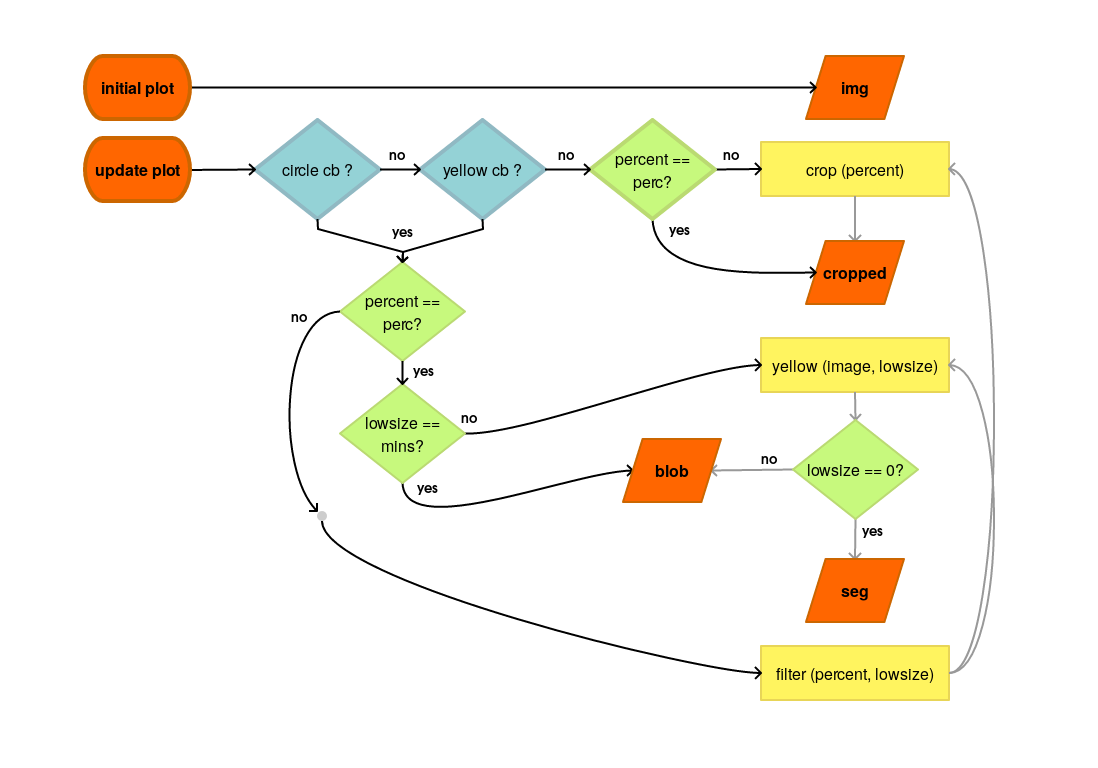
\includegraphics[width=\textwidth,angle=0]{abb/prozess-flow}
 \caption{Programm flowchart}
\label{fig:flowchart}
\end{figure}

Die inneren Prozesse einer Plotabfrage werden in Abbildung \ref{fig:flowchart} (S.\pageref{fig:flowchart}) dargestellt. Hauptintention dabei stellt die Minimierung von Zeitverzögerungen da. Vor Allem die Wiederholung von unnötigen Berechnungen soll durch if-else Schleifen vermieden werden. Es werden je nach Prozess der berechnet wird zunächst erstmal abgefragt, ob sich die Parameter überhaupt verändert haben. 
Ist dies nicht oder nur teilweise der Fall kann eine erneute komplette Berechung nicht notwenig sein und der angefragte Prozess auf ein schon gespeichertes Bild oder eine Teilfunktion direkt zurückgreifen kann. Der Aufruf des Gesamtfilters, der die gelben Bildteile mit einer Mindestgröße segmentiert, ruft Funktionen auf, die jeweils auch direkt von anderen Anfragen angesprochen werden können. Dabei werden die Zwischenergebnisse als Objekte der Klasse gespeichert. Insgesamt kann so die Ausgabe effizienter und schneller wiedergegeben werden, gerade bei Bilder, die eine große Dateimenge einnehmen.

\subsection{Vorgehensweise Methoden?}

genaue Beschreibung der Methoden (Wie wird der Bereich heraus gefiltert, Datenstruktur?, GUI, Parameter)
nach welchen Kriterien und warum diese gewählt -> Quellen?

Methoden: 
- Filtern nach Farbebereich ->
Allen Bildpunkten, die nicht in dem Farbbereich zwischen RGB (200, 133, 0) und (255, 255, 122) liegen, wird mit der Hilfe einer Maske 0 zugeordnert. 

- 

% dafür wird das Bild als dreidimensioneller BGR-Array mit je einer Ebene je Farbband. Mit der Funktion cv2.inRange() wird eine Maske erstellt, die für alle Pixel, die nicht in dem Bereich sind 0 zuordnet und für alle die in dem Bereich sind 255. Diese Maske lässt sich auf das originale Bild mit cv2.bitwise() übertragen. Dabei werden zwei Bilder zusammengefügt, im Bereich einer Maske.??doppelt?? 
Warum nach Farbbereich filter:
strong argument -> Starkes Charakteristika der Arnika Blume ist die Farbe. Dies als erstes Erkennungsmerkmal gewählt.


Datenstruktur:
Dazu einleitung: Objektorientierte Programmierung, vorteile?
Es gibt die Data class, die ein Bild als Instanz lädt und deren Objekte die durch Methoden veränderte Bilder sind. 
DesignerMainWindow class als gesamt GUI, die dann alle anderen Dinge "erbt" bzw. aufruft.
Es gibt das MplWidget als class, die die Canvas class aufruft und das Plotfenster bildet und Teil der Gui ist. 
Gui mit pyqt5 Backend geschrieben und mit dem Qt5Designer erstellt.

\subsubsection{Parameterbeschreibung}


\subsection{Implementierung / Aufruf}    
% Flow-Chart für die GUI und den Programmaufruf, quasi als "Anleitung der Benutzung"

% Beschreibung der genauen Eingabe, wie im ersten Abschnitt mit den Gui-screenshots schon angefangen. 

%Navigationtoolbar beschreiben: 
%https://github.com/matplotlib/matplotlib/blob/master/doc/users/navigation_toolbar.rst


\subsubsection{Hard- und Softwarevoraussetzungen}
\subsubsection{(Notwendige) In- und Output-Dateien und deren Formate}



- Einbindungsmöglichkeiten in andere Anwendungen
- Bei komplexen Berechnungsverfahren Beschreibung der Algorithmen und Literaturhinweise zu den Quellen der Verfahren


    

\newpage
\section{Ergebnisse}

Einleitende Zusammenfassung etc.
\subsection{Auswertung}
Alle Ergebnisse werden hinsichtlich der Zielsetzung (Anfangshypothesen) bewertet
Alle Ergebnisse werden mit relevanter Literatur verglichen und bewertet


\subsection{Schwierigkeiten}
\subsubsection{Problem: Kreise um zusammenhängende Blumen}

Bei der Visualisierung der Blumen durch Kreise gibt es ein Problem, wenn mehrere Blumen zusammenhängen. 
Bei einer Gruppe von Blüten, die überlappen, wird ein zusammenhängende Fläche (ConnectedComponents) bei der gelben Segmentierung heraus gefiltert. Möchte man die Blumen mit Kreisen visualisieren wird der Geometrischer Schwerpunkt der Connected Components (CC) als Mittelpunkt des Kreises gewählt. Als Radius wurde die Höhe oder Breite des CC gewählt, je nachdem welche geringer ist. Hängen nun aber mehrerer Blüten zusammen kann nur ein Kreis mit den Mittelpunkt des gesamten CC gezeichnet werden (Siehe Abbildung~\ref{fig:Kreis}, S. \pageref{fig:Kreis}).
 
\begin{figure}[htb]
 \centering
 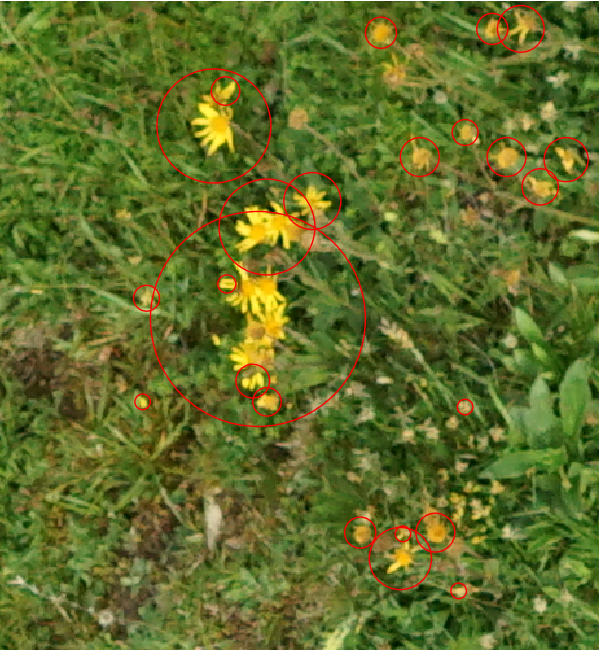
\includegraphics[width=0.4\textwidth,angle=0]{abb/ergebnisse/probleme/bigblob}
 \caption{Ein großer Kreis um zusammenhängende Blumen}
\label{fig:Kreis}
\end{figure}

\paragraph{Lösungsansatz:}
Anstatt einfach den Bildschwerpunkt, der von der Statistik der ConnectedComponents Funktion von OpenCV geliefert wird, wurde versucht die großen CC in ihrem Seitenverhältnis von Höhe zu Breite bzw. Breite zu Höhe zu teilen und mehrere Mittelpunkte anzulegen. 

Idee: center der Kreise bei 1:2, 1:3, 1:4 und 1:5 Verhältnis von Höhe /Breite bzw. Breite zu Höhe verschieben und duplizieren,


\begin{figure}[htb]
 \centering
 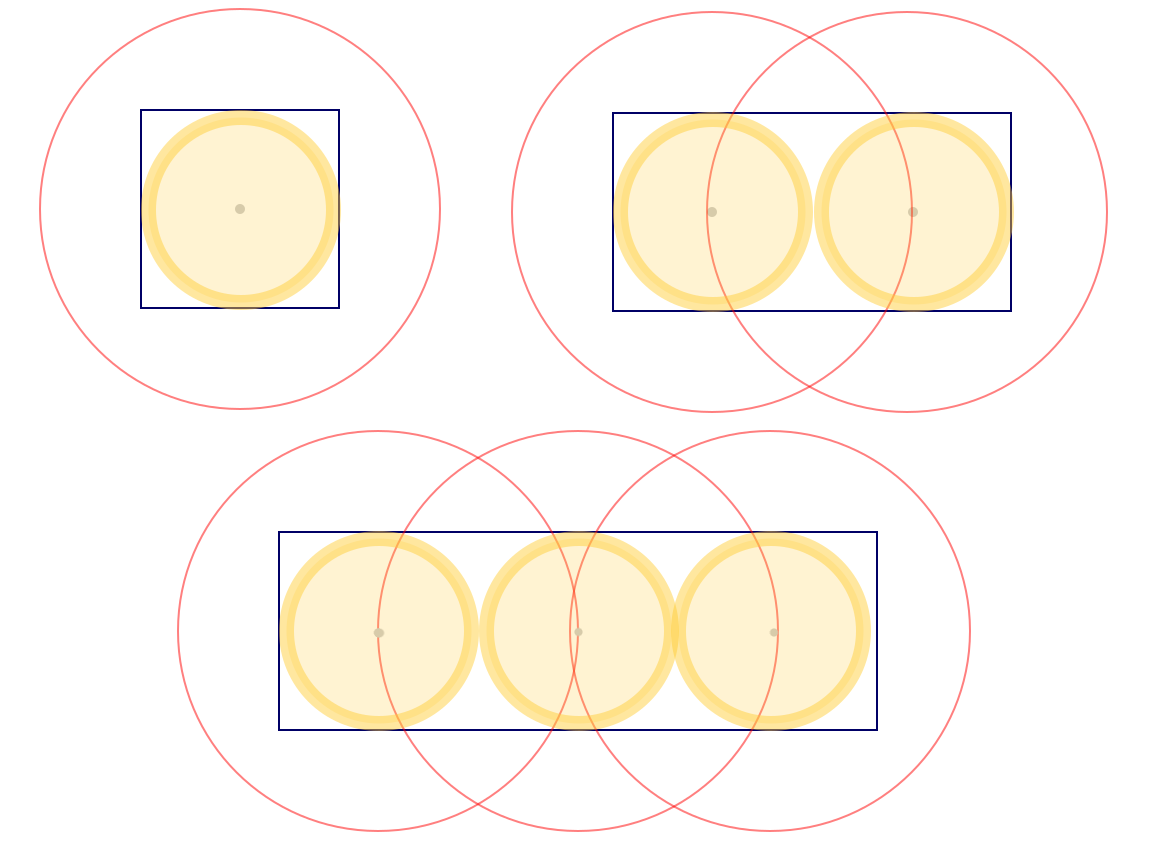
\includegraphics[width=0.5\textwidth,angle=0]{abb/ergebnisse/probleme/seitenverhaeltnis}
 \caption{Schematische Darstellung verschiedener Seitenverhätnisse}
\label{fig:Schema}
\end{figure}


Problem dabei: Wenn eine einzelne Blume aber nicht frontal sondern eher seitlich aufgenommen wurde, hat sie auch dieses Seitenverhältnis und wird auch doppelt gezählt.

\begin{figure}[htb]
 \centering
 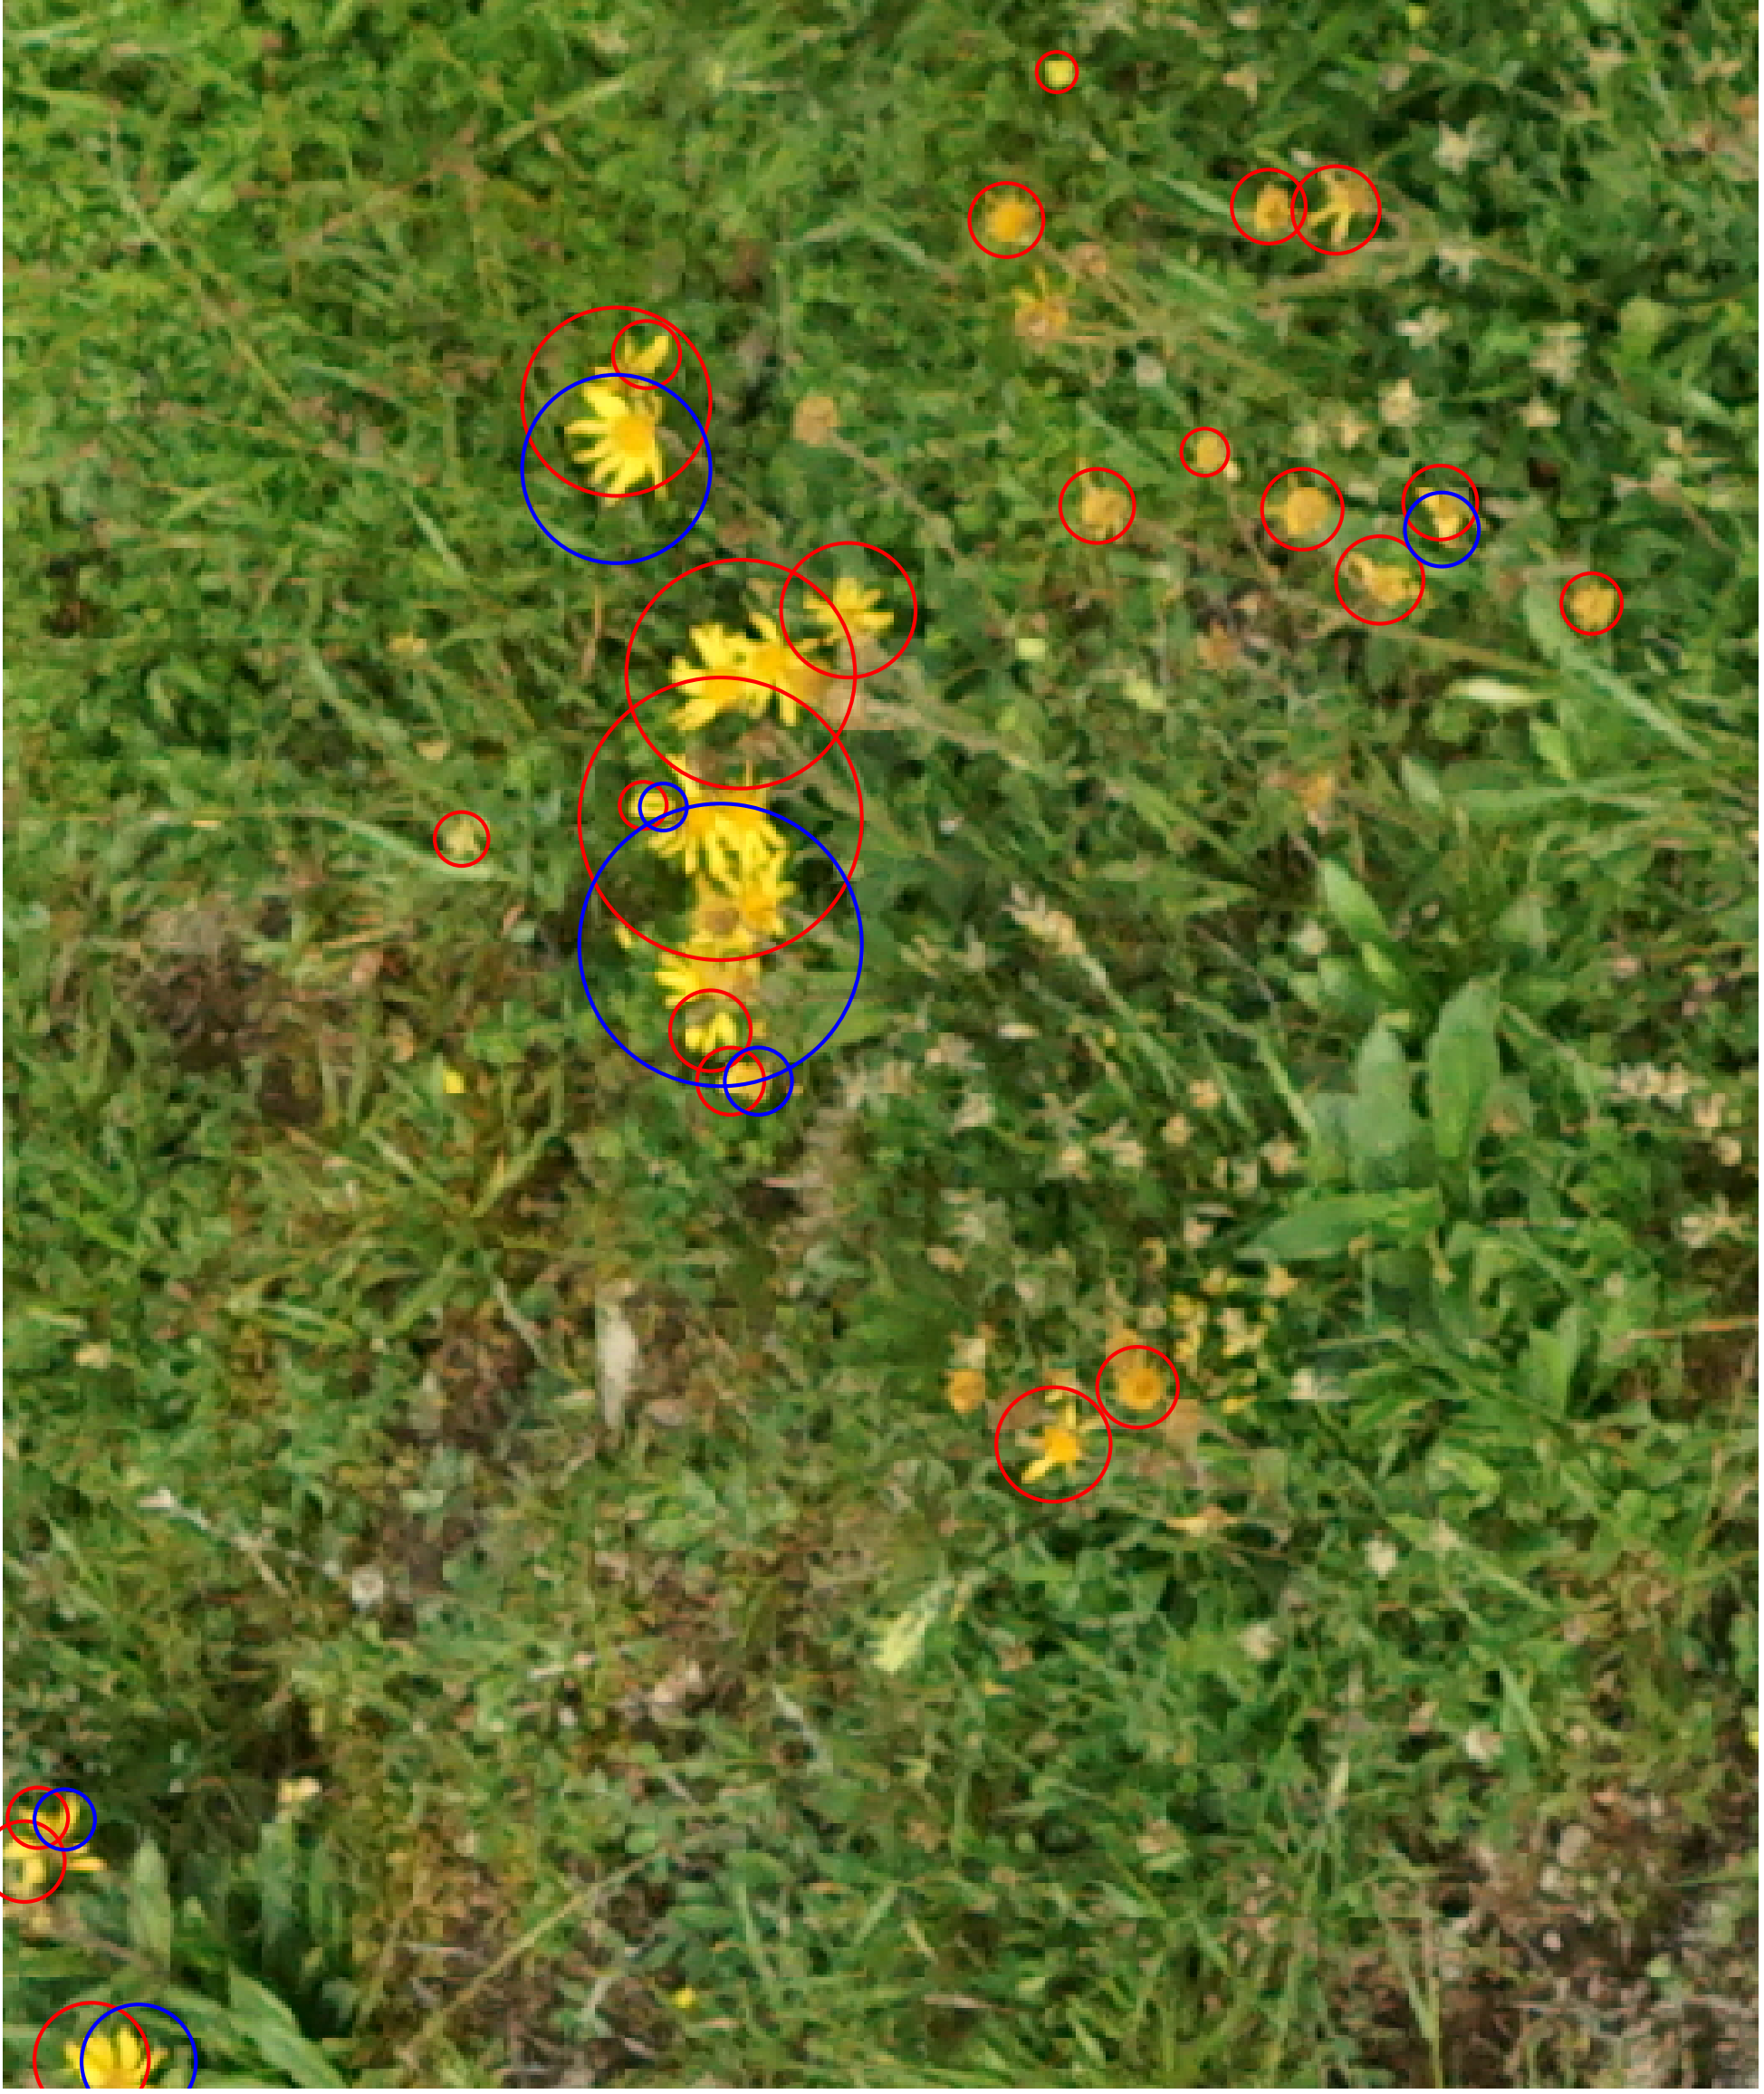
\includegraphics[width=0.4\textwidth,angle=0]{abb/ergebnisse/probleme/circles}
 \caption{Kreise bei nicht proportionalen CC hinzugefügt (blau)}
\label{fig:Kreis-blau}
\end{figure}

Also müsste man das Seitenverhältnis mit der Größe der CC kombinieren. Also die Analyse des Seitenverhältnisses nur bei einer bestimmten Größe beginnen. 
also nicht nur max size, sondern if size > maxsize: die center hinzufügen?

\blindtext
\lstset{language=python}
\begin{lstlisting}[frame=htrbl, caption={Das Listing zeigt Python Quellcode}, label={lst:result2}]
number, output, stats, centroids = cv2.connectedComponentsWithStats(test.blob[:, :, 0], connectivity=8)

width = stats[1:,2]
height = stats[1:,3]
sizes = stats[1:,4]
number = number - 1
lowsize = np.mean(sizes)*2

center = np.array((centroids[1:, 0].astype(int), centroids[1:, 1].astype(int))).transpose()

centers = []
radius = []
for i in range(0, number):
    if sizes[i] >= lowsize:
        if width[i]/height[i] >= 0.75 and width[i]/height[i] < 1.5:
            # 1:1 do nothing
            pass
        elif width[i]/height[i] < 0.75 and width[i]/height[i] >= 0.415:
            center[i] = np.array([(width[i] / 2) + stats[i + 1, 0], (height[i] / 4) + stats[i + 1, 1]])
            centers.append([(width[i] / 2) + stats[i + 1, 0], (height[i] / 4) * 3 + stats[i + 1, 1]])
            radius.append(np.min(stats[i + 1, 2:4]))
\end{lstlisting}

\begin{figure}[htb]
 \centering
 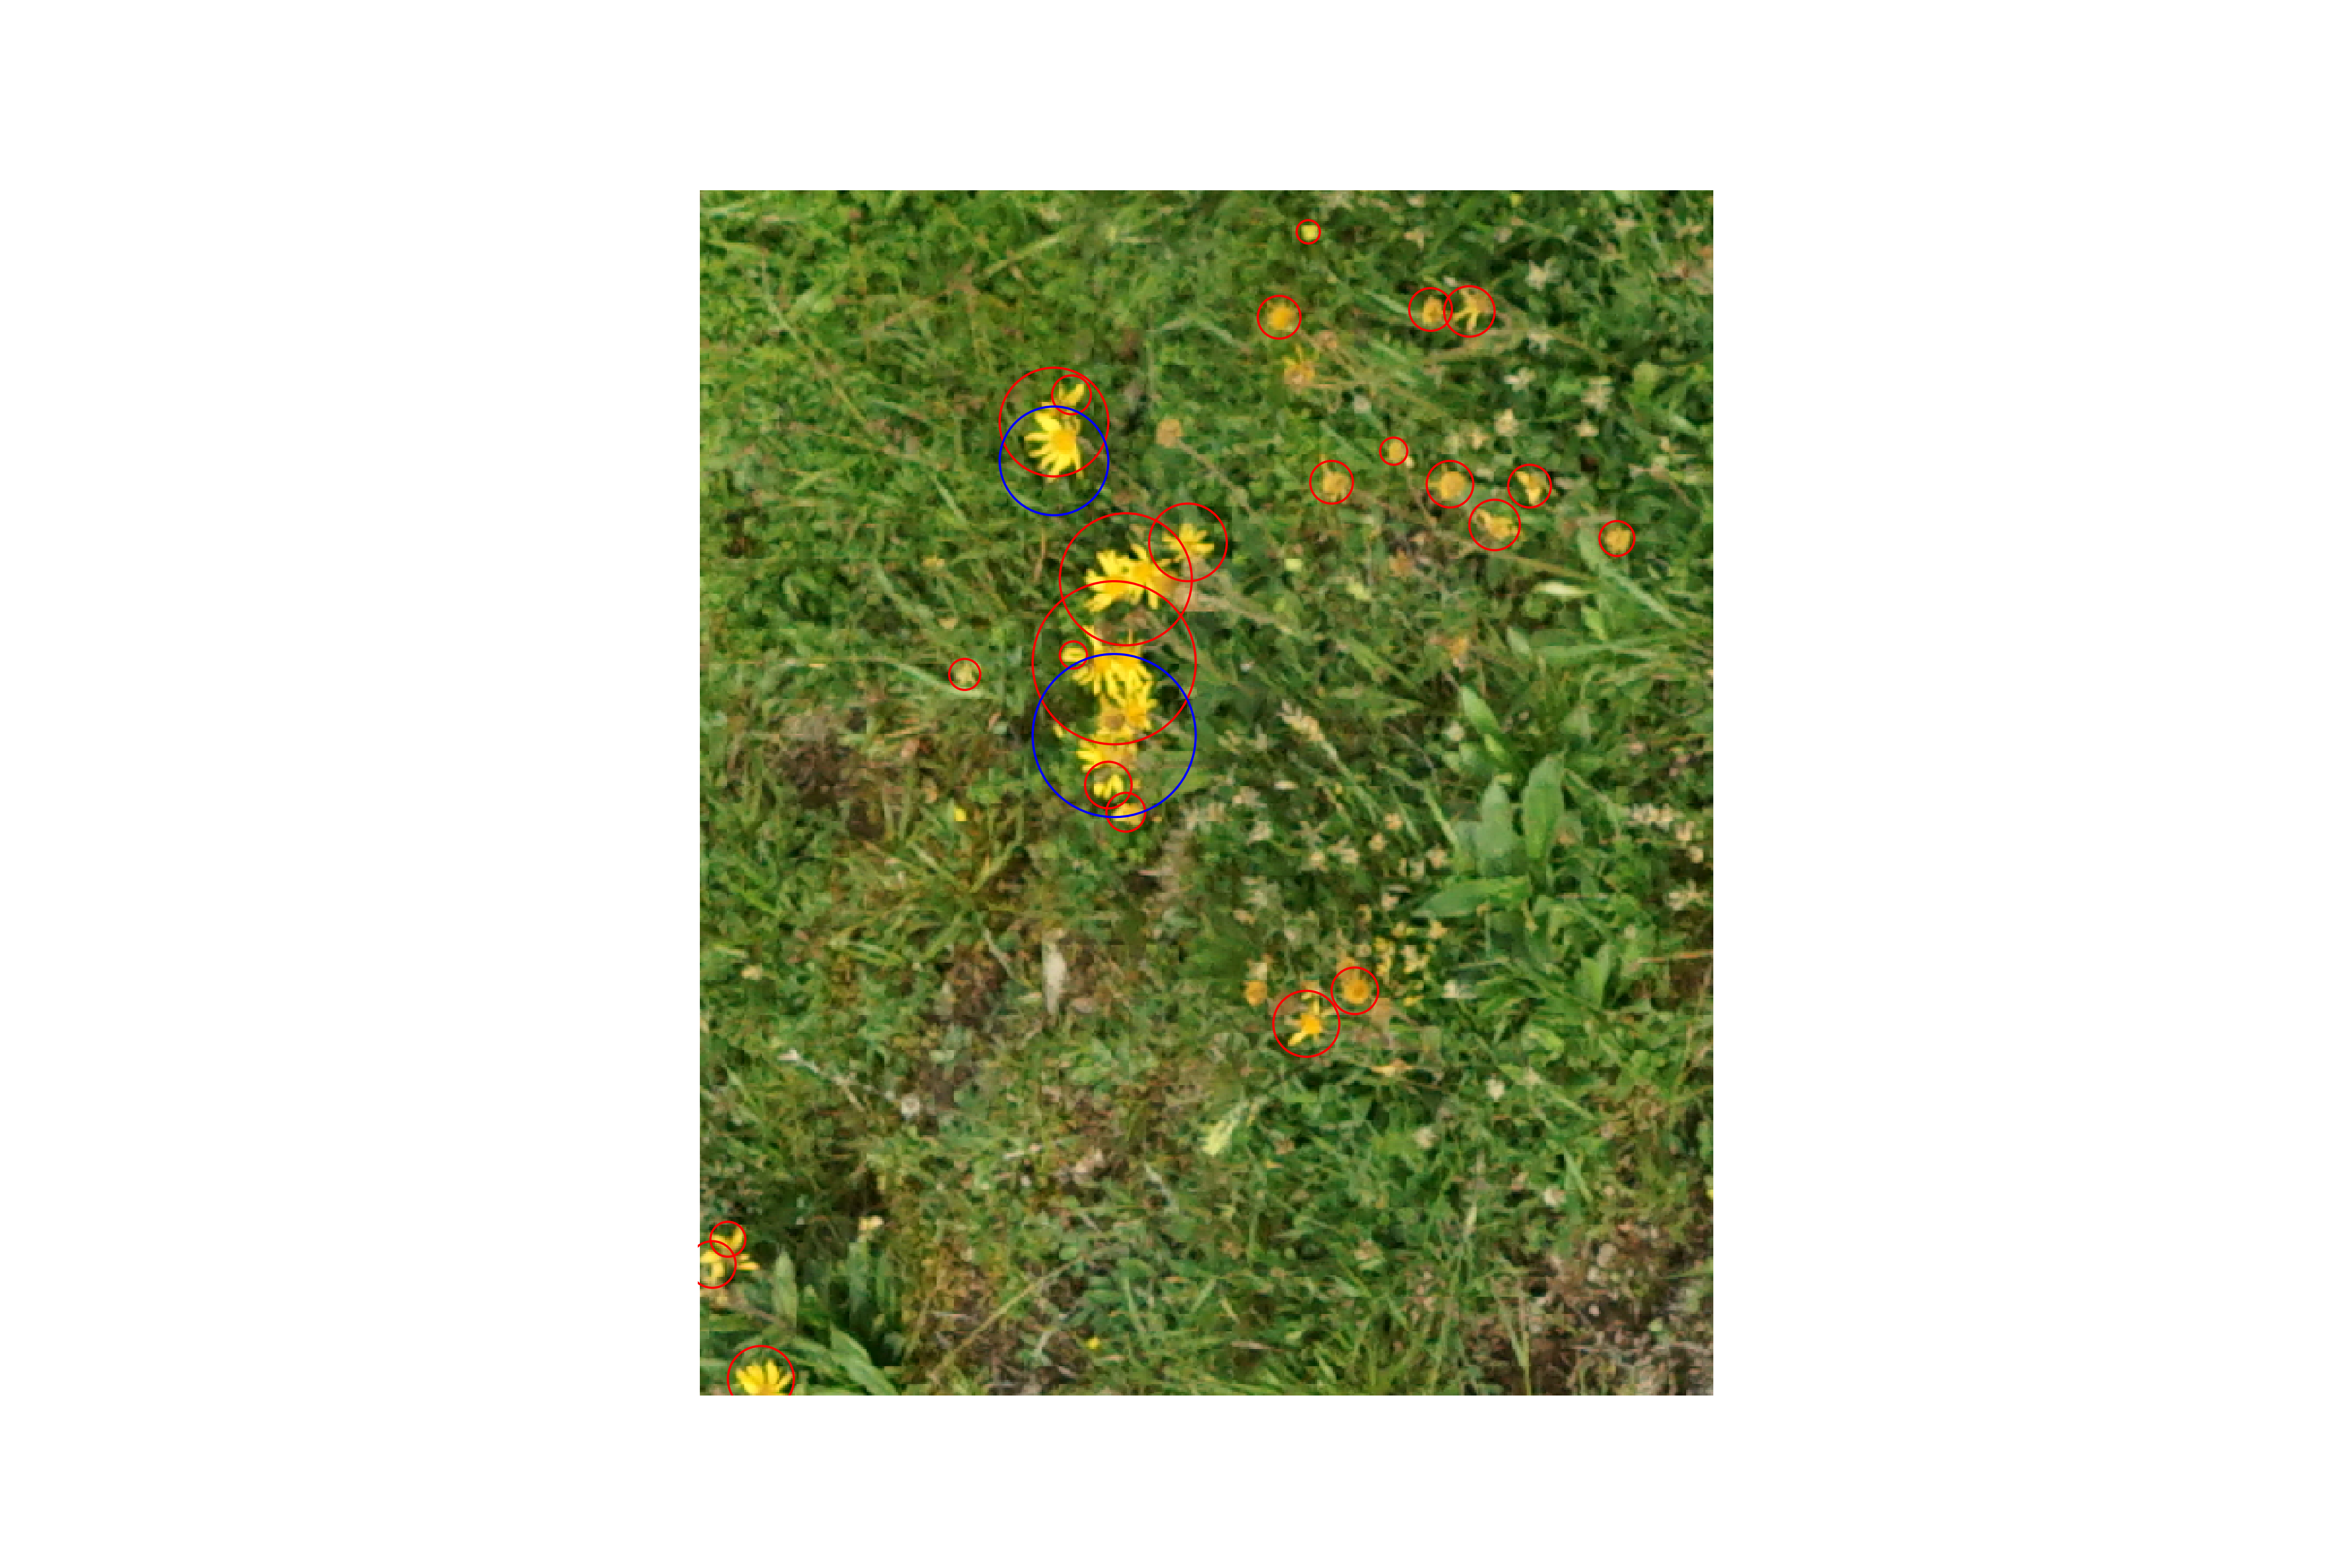
\includegraphics[width=0.4\textwidth,angle=0]{abb/ergebnisse/probleme/circles-adjust}
 \caption{Kreise nur bei großen CC hinzugefügt (blau)}
\label{fig:Kreis-blau2}
\end{figure}

Kritische Reflektion, ob das so erfolgreich war...

\subsubsection{Problem: Blume wird durch Schatten gestückelt}

Idee: Smoothing edges vor segmentation um trennungen der Blüten rückgängig zu machen


Verbesserungsmöglichkeiten
Die eigenen Ergebnisse werden nicht über- oder unterbewertet

\subsubsection{Problem: Verwechslungspotential Arnica montana}

 schwer zu verhindern, aber durch andere faktoren identifikation -> GSM und Höhe der Pflanzen oder Bodensäure?


\newpage
%\section{Diskussion}\label{diskussion}

\newpage

\section{Fazit}\label{fazit}


%% Beispiel für Bild mit Fußnote
\begin{figure}[htb]
 \centering
 %\includegraphics[width=0.4\textwidth,angle=45]{abb/logo1}
 \caption[Beispiel einer Bildbeschreibung]{Beispiel einer Bildbeschreibung\footnotemark}
\label{fig:beispiel1}
\end{figure}
\footnotetext{Bildquelle: Beispielquelle}

% Beispiel für Bildintegration
\begin{figure}[htb]
 \centering
 %\includegraphics[width=0.3\textwidth,angle=0]{abb/logo2}
 \caption[Beschreibung]{Beschreibung}
\label{fig:Beschreibung}
\end{figure}

% Beispiel: Referenz auf Abbildung
%Abbildung~\ref{fig:Beschreibung} [S.\pageref{fig:Beschreibung}]

% Beispiel: Tabelle 
\begin{center}
  \begin{tabular}{ | l | c | }
    \hline
    Überschrift 1 & Überschrift 2 \\ \hline \hline
    Info 1 & Info 2 \\ \hline
    Info 3 & Info 4 \\
    \hline
  \end{tabular}
\end{center}



\lstset{language=java}
\begin{lstlisting}[frame=htrbl, caption={Das Listing zeigt Java Quellcode}, label={lst:result2}]
/* generate TagCloud */
Cloud cloud = new Cloud();
cloud.setMaxWeight(_maxSizeOfText);
cloud.setMinWeight(_minSizeOfText);
cloud.setTagCase(Case.LOWER);
	    
/* evaluate context and find additional stopwords */
String query = getContextQuery(_context);
List<String> contextStoplist = new ArrayList<String>();
contextStoplist = getStopwordsFromDB(query);
	    
/* append context stoplist */
while(contextStoplist != null && !contextStoplist.isEmpty())
  _stoplist.add(contextStoplist.remove(0));
	    
/* add cloud filters */
if (_stoplist != null) {
  DictionaryFilter df = new DictionaryFilter(_stoplist);
  cloud.addInputFilter(df);
}
/* remove empty tags */
NonNullFilter<Tag> nnf = new NonNullFilter<Tag>();
cloud.addInputFilter(nnf);

/* set minimum tag length */
MinLengthFilter mlf = new MinLengthFilter(_minTagLength);
cloud.addInputFilter(mlf);

/* add taglist to tagcloud */
cloud.addText(_taglist);

/* set number of shown tags */	    
cloud.setMaxTagsToDisplay(_tagsToDisplay);
\end{lstlisting}


% Beispiel für Formeln
Die Zuordnung aller möglichen Werte, welche eine Zufallsvariable annehmen kann nennt man \emph{Verteilungsfunktion} von $X$.

\begin{quotation}
Die Funktion F: $\mathbb{R} \rightarrow$ [0,1] mit $F(t) = P (X \le t)$ heißt Verteilungsfunktion von $X$.\footnote{Konen, vgl.}
\end{quotation}

\begin{quotation}
Für eine stetige Zufallsvariable $X: \Omega \rightarrow \mathbb{R}$ heißt eine integrierbare, nichtnegative reelle Funktion $w: \mathbb{R} \rightarrow \mathbb{R}$ mit $F(x) = P(X \le x) = \int_{-\infty}^{x} w(t)dt$ die \emph{Dichte} oder \emph{Wahrscheinlichkeitsdichte} der Zufallsvariablen $X$.\footnote{Konen, vgl.~}
\end{quotation}


\onecolumn
% einfacher Zeilenabstand
\singlespacing
% Literaturliste soll im Inhaltsverzeichnis auftauchen
\newpage
\addcontentsline{toc}{section}{Literaturverzeichnis}
% Literaturverzeichnis anzeigen
\renewcommand\refname{Literaturverzeichnis}
\bibliography{jabbib}

%% Index soll Stichwortverzeichnis heissen
% \newpage
% % Stichwortverzeichnis soll im Inhaltsverzeichnis auftauchen
% \addcontentsline{toc}{section}{Stichwortverzeichnis}
% \renewcommand{\indexname}{Stichwortverzeichnis}
% % Stichwortverzeichnis endgueltig anzeigen
% \printindex

\onehalfspacing
% evtl. Anhang
\newpage
\addcontentsline{toc}{section}{Anhang}
%\fancyhead[L]{Anhang} %Kopfzeile links
\subsection*{Anhang}\label{anhang}


% Eidesstattliche Erklärung
\addcontentsline{toc}{section}{Eidesstattliche Erklärung}
\section*{Eidesstattliche Erklärung}
\thispagestyle{empty}

\begin{verbatim}

\end{verbatim}

\begin{LARGE}Eidesstattliche Erklärung zur <-Arbeit>\end{LARGE}
\begin{verbatim}


\end{verbatim}
Ich versichere, die von mir vorgelegte Arbeit selbstständig verfasst zu haben. Alle Stellen, die wörtlich oder sinngemäß aus veröffentlichten oder nicht veröffentlichten Arbeiten anderer entnommen sind, habe ich als entnommen kenntlich gemacht. Sämtliche Quellen und Hilfsmittel, die ich für die Arbeit benutzt habe, sind angegeben. Die Arbeit hat mit gleichem Inhalt bzw. in wesentlichen Teilen noch keiner anderen Prüfungsbehörde vorgelegen.



\begin{displaymath}
% use packages: array
\begin{array}{ll}
Unterschrift:~~~~~~~~~~~~~~~~~~~~~~~~~~~~~~~~~~~~~~~~~~
& Ort, Datum:~~~~~~~~~~~~~~~~~~~~~~~~~~~~~~~~~~~~~~~~~~
\end{array}
\end{displaymath}


% leere Abschlussseite
\newpage
\thispagestyle{empty} % erzeugt Seite ohne Kopf- / Fusszeile
\section*{ }

\end{document}
